\documentclass{article}

\usepackage{graphicx}
\usepackage{physics}
\usepackage{subcaption}
\usepackage{hyperref}
\usepackage{float}

\usepackage[left=2.5cm, right=2.5cm, top=2.5cm, bottom=2.5cm]{geometry}
\setlength{\parindent}{0em}
\setlength{\parskip}{0.8em}

\usepackage{caption}
\captionsetup{width=.9\textwidth}

\usepackage{biblatex}
\addbibresource{report.bib}

\title{Exam, TFY4235 Computational physics}
\author{Number}
\vspace{-8ex}
\date{}


\begin{document}
    \maketitle
    \section*{Introduction}
    SIR, and the more advanced SEIIaR, are mathematical models that aim to capture how pandemics spread throughout a simulation.
    This paper documents the implementation and results of the simulation of these models in Python, as described in \cite{exam}.

    \section*{Implementation}
    All the different models used in this text follow the same basic form. 
    The goal is to find $x(t)$, given initial conditions $x(t_0)$, and a equation of the form
    \begin{equation*}
        f(x(t); \mathrm{args}) = \dv{x(t)}{t}.
    \end{equation*}
    In the first part, $x = (S, I, R)$, while later $x = (S_{ij}, E_{ij}, I_{ij}, Ia_{ij}, R_{ij})$ where $(ij)$ are different population groups. 
    This is accomplished using function \verb|integrate| in \verb|utilities.py|. 
    It takes as arguments the initial conditions \verb|x0|, the functions \verb|f| and \verb|step|, the list \verb|args| as well as the time step \verb|dt| and total time \verb|T| to simulate. 
    It then creates a discrete approximation of $x(t)$ by taking time steps given by the function \verb|step|. 
    \verb|step| is the particular \emph{scheme} used, for example Runge-Kutta (4,5), while \verb|f| defines the system. 


    The equations that give the asymptotic behavior are both of the type $x = f(x)$, and can thus be approximated by recursion, given that they converge. 
    For $\mathcal{R}_0$ close to one, they converge increasingly slowly, and the program may reach maximum recursion depth. 
    For the parameters in this exercise, however, this was not a problem

    \section*{Results}
    \subsection*{Deterministic SIR model}
    The first model is the deterministic SIR model, given by a set of coupled ODEs \cite{exam}. 
    In this text, the Runge-Kutta (4, 5) scheme was used, as it is both a simple yet precise scheme.
    \autoref{SIR} demonstrates that $S$ and $R$ approaches the expected asymptotes, and that $I$ grows exponentially in the beginning, at the rate expected.
    \autoref{conv det} shows an error estimation of different integration schemes.
    The error is found by comparing to a solution found by using the RK4-solver, and $\Delta t = 0.01$.
    This illustrates why the choice of $\Delta t = 0.1$ is sufficient, as numerical errors start playing a large role for larger $\Delta t$.
    
    Adjusting the $\beta$-parameter will affect how fast the virus spreads, thus ``flattening the curve'', as illustrated in \autoref{flattening}.
    This shows that the highest $\beta$ that still keeps the maximum fraction of population being infected at once below $20\%$ is $\beta=0.23$. 
    \autoref{vax} shows the fraction of the population must be vaccinated \emph{before} the outbreak to stop exponential growth. 
    At the start of the simulation, the number of infected grows exponentially, i.e. $I \propto \exp(\alpha t)$ for some $\alpha$.
    A partially vaccinated population can be modeled by setting $R(0)$ equal the proportion of the population that is vaccinated.
    The result shows that $60\%$ or more must be vaccinated to avoid exponential growth, i.e. $\alpha\leq 0$. 
    These results could be made more precise by extrapolation, more simulation or searching with the bisection method, but the crudeness of the model means higher precision is wasted.

    \begin{figure}[H]
        \centering
        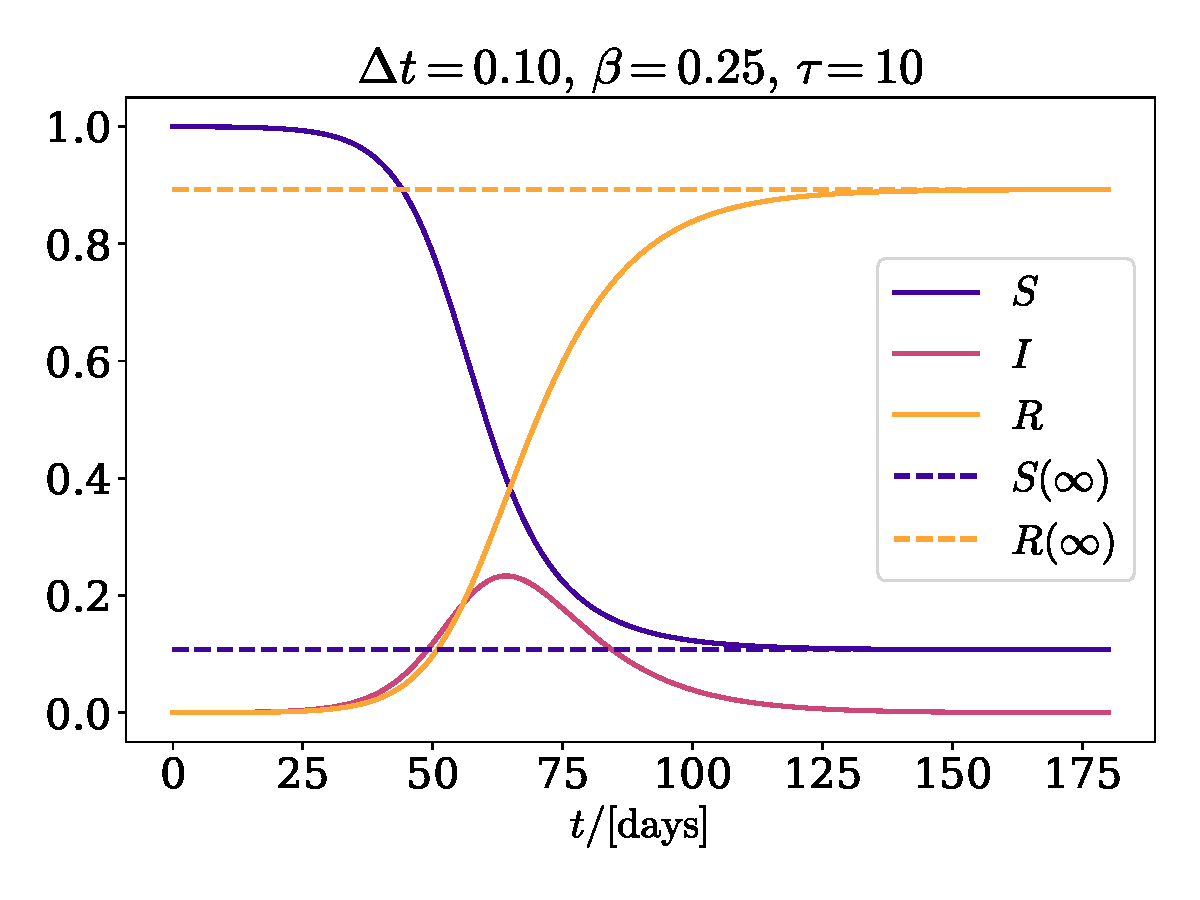
\includegraphics[width=.49\textwidth]{../plots/2A/TestSIR}
        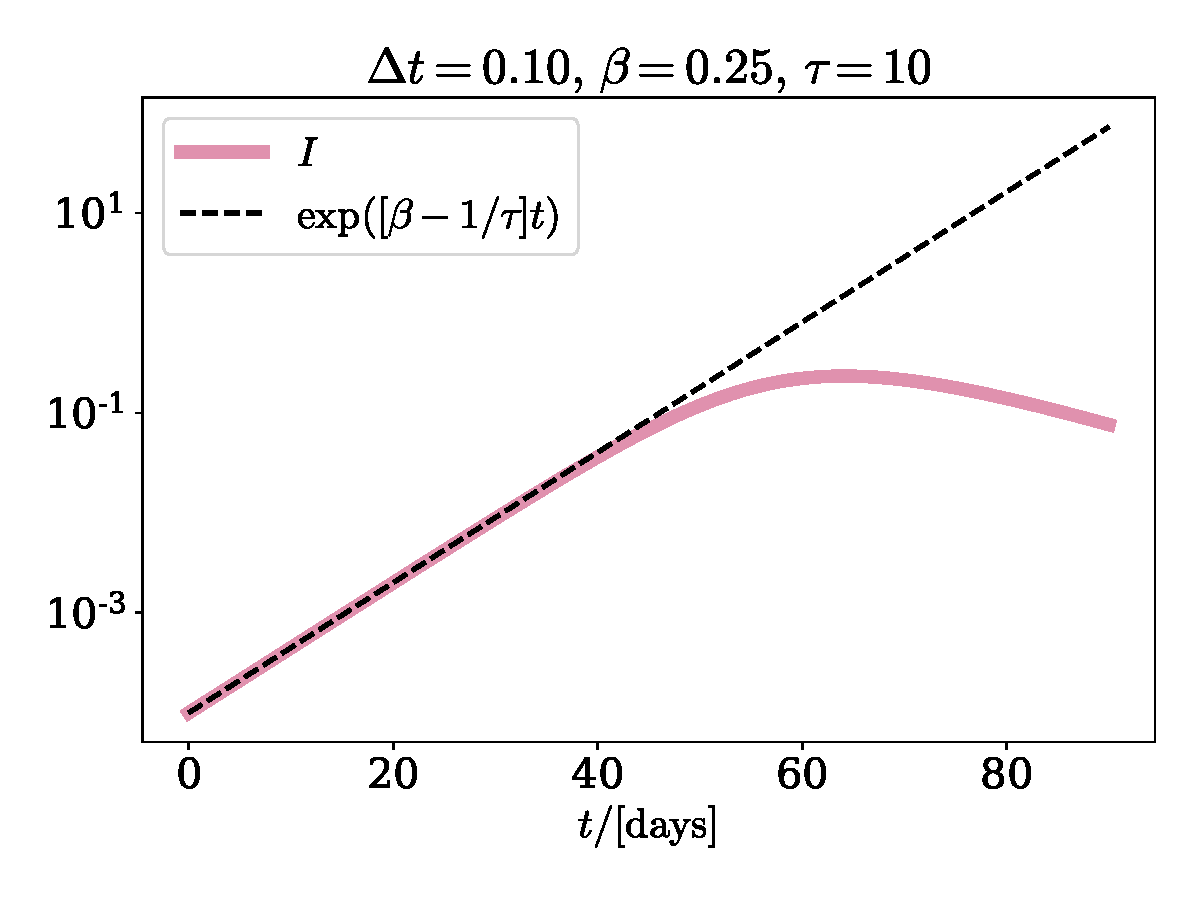
\includegraphics[width=.49\textwidth]{../plots/2A/TestI}
        \caption{On the left, the fraction of the population that is in each group, over time. The plot on the right shows how the infection spreads exponentially in the begining}
        \label{SIR}
    \end{figure}

    \begin{figure}[H]
        \centering
        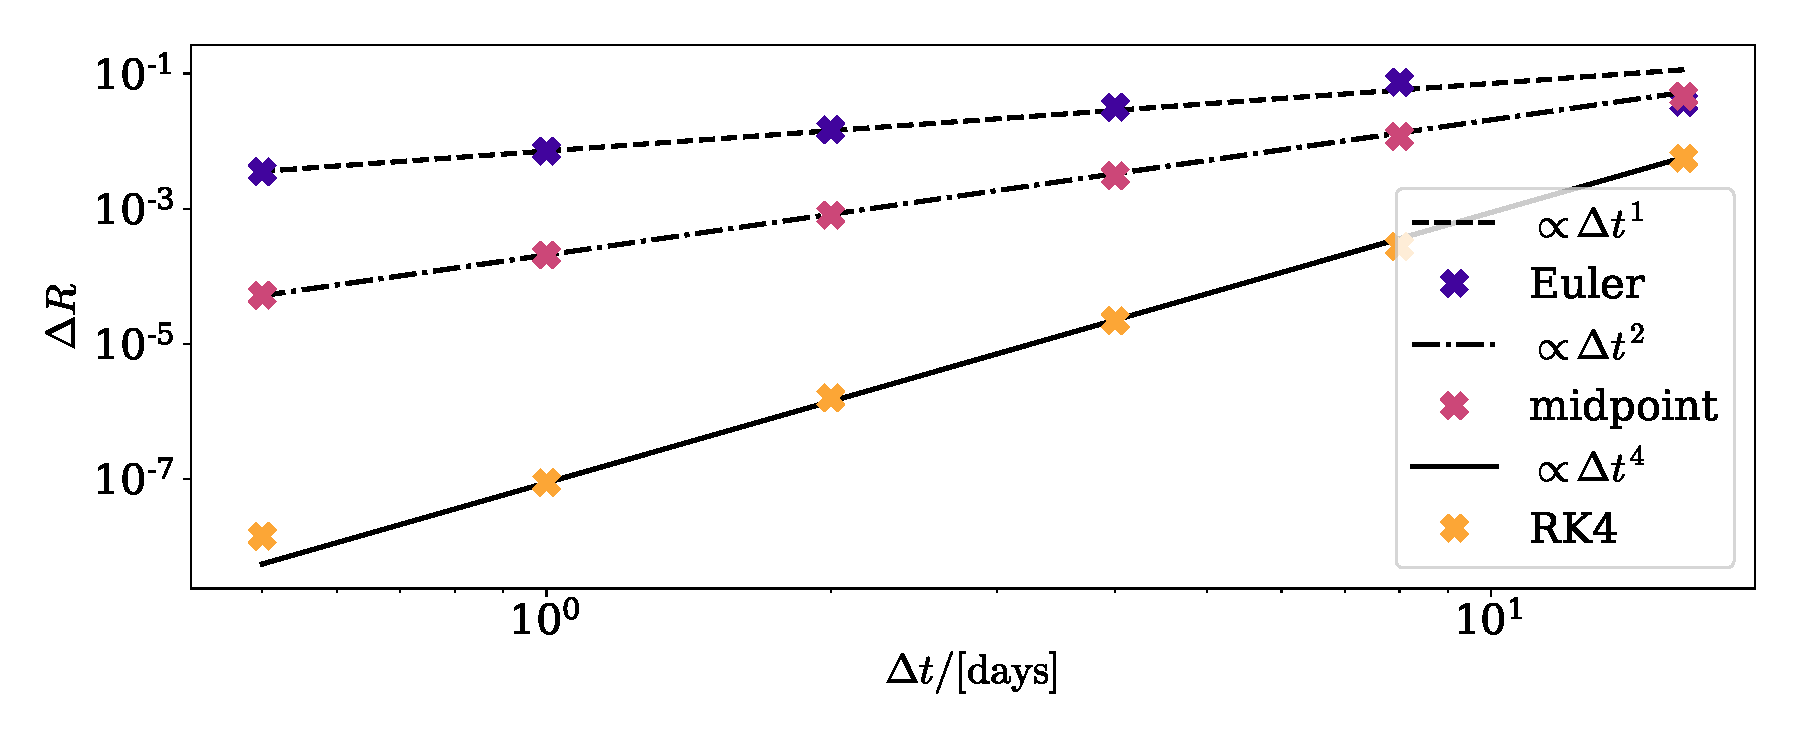
\includegraphics[width=.6\textwidth]{../plots/2A/conv}
        \caption{The error, after, 128 days, of different integration schemes. All are compared with RK4, with steplength $\Delta t = 0.01$.}
        \label{conv det}
    \end{figure}

    \begin{figure}[H]
        \centering
        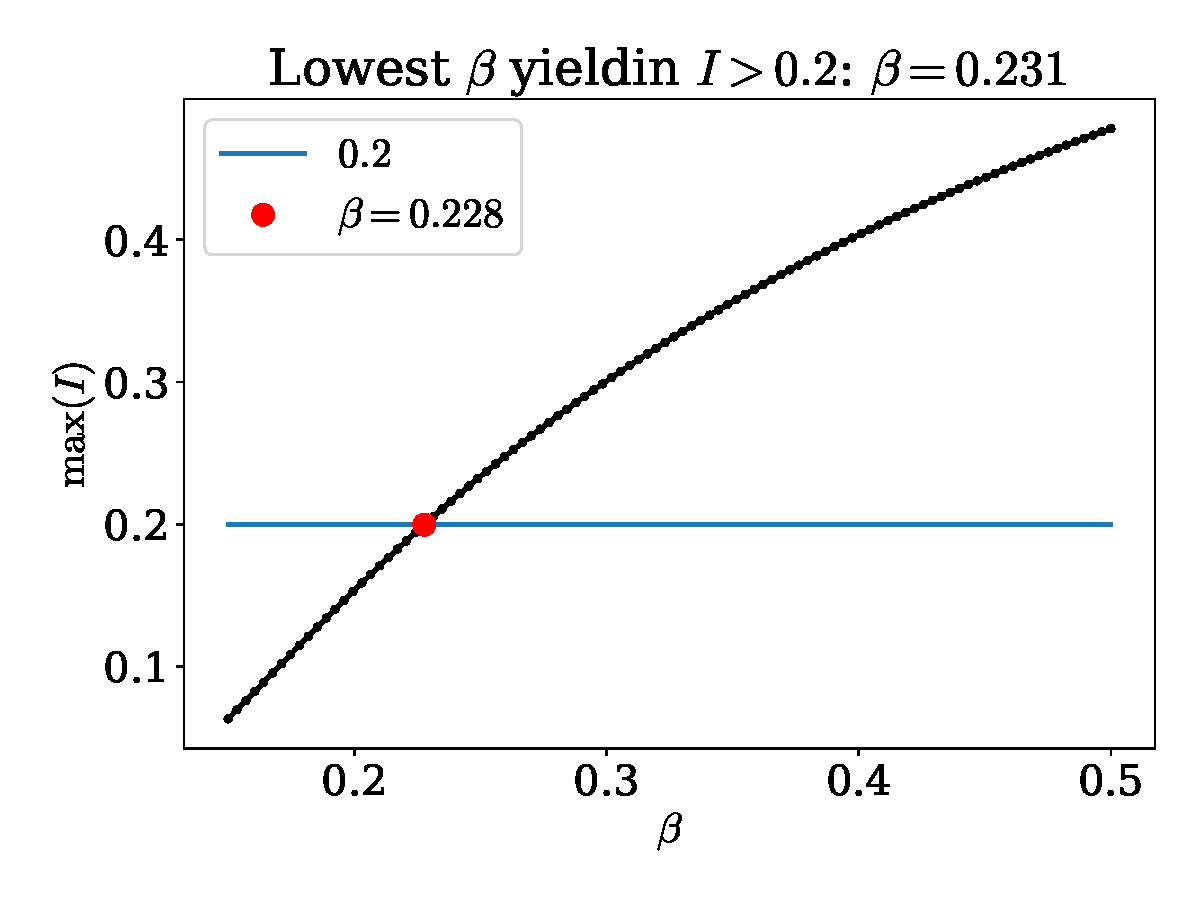
\includegraphics[width=.49\textwidth]{../plots/2A/flatten.pdf}
        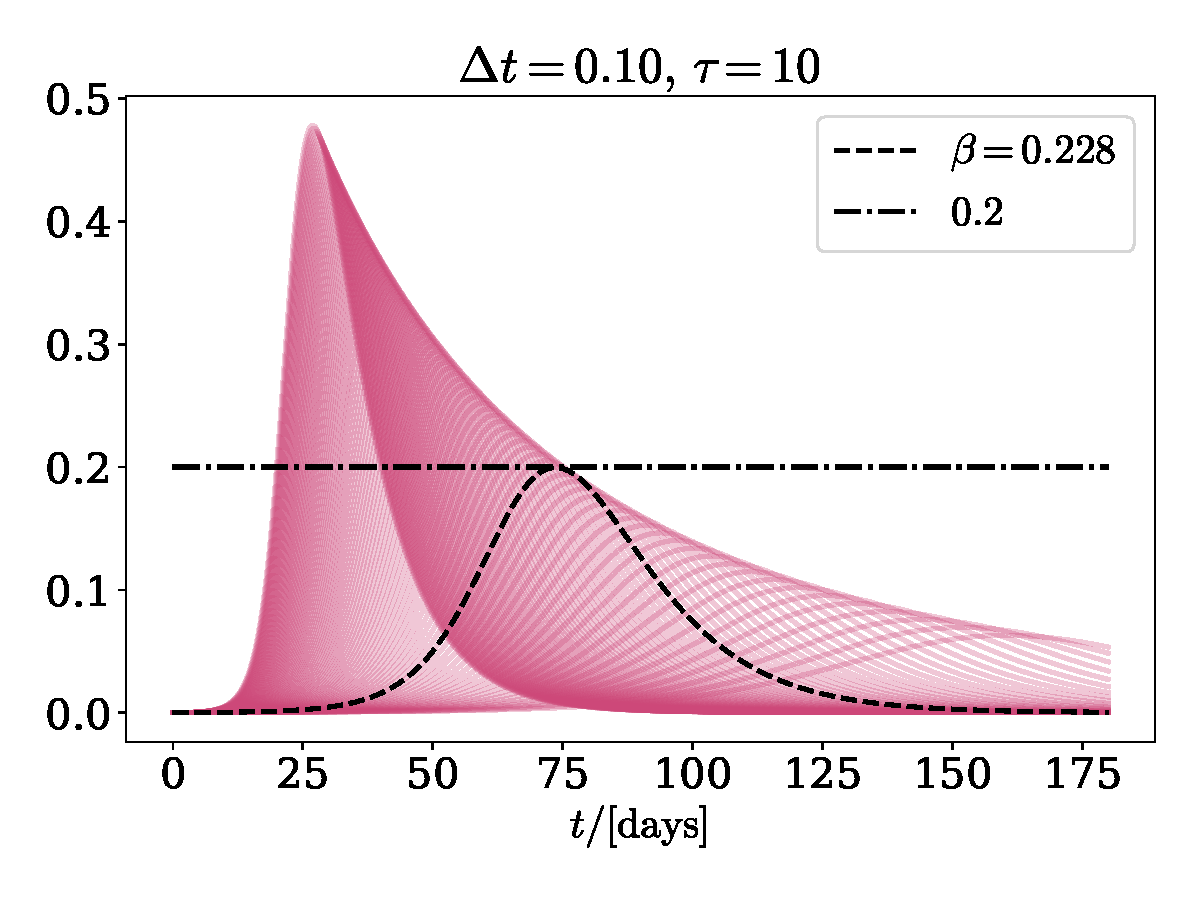
\includegraphics[width=.49\textwidth]{../plots/2A/flattenIs.pdf}
        \caption{The figure on th eright shows the maximum fraction of infected, as a function of $\beta$. The largest value of $\beta$ such that the maximum is beneth $0.2$ is indicated. On the right, the corresponding infection curves.}
        \label{flattening}
    \end{figure}

    \begin{figure}[H]
        \centering
        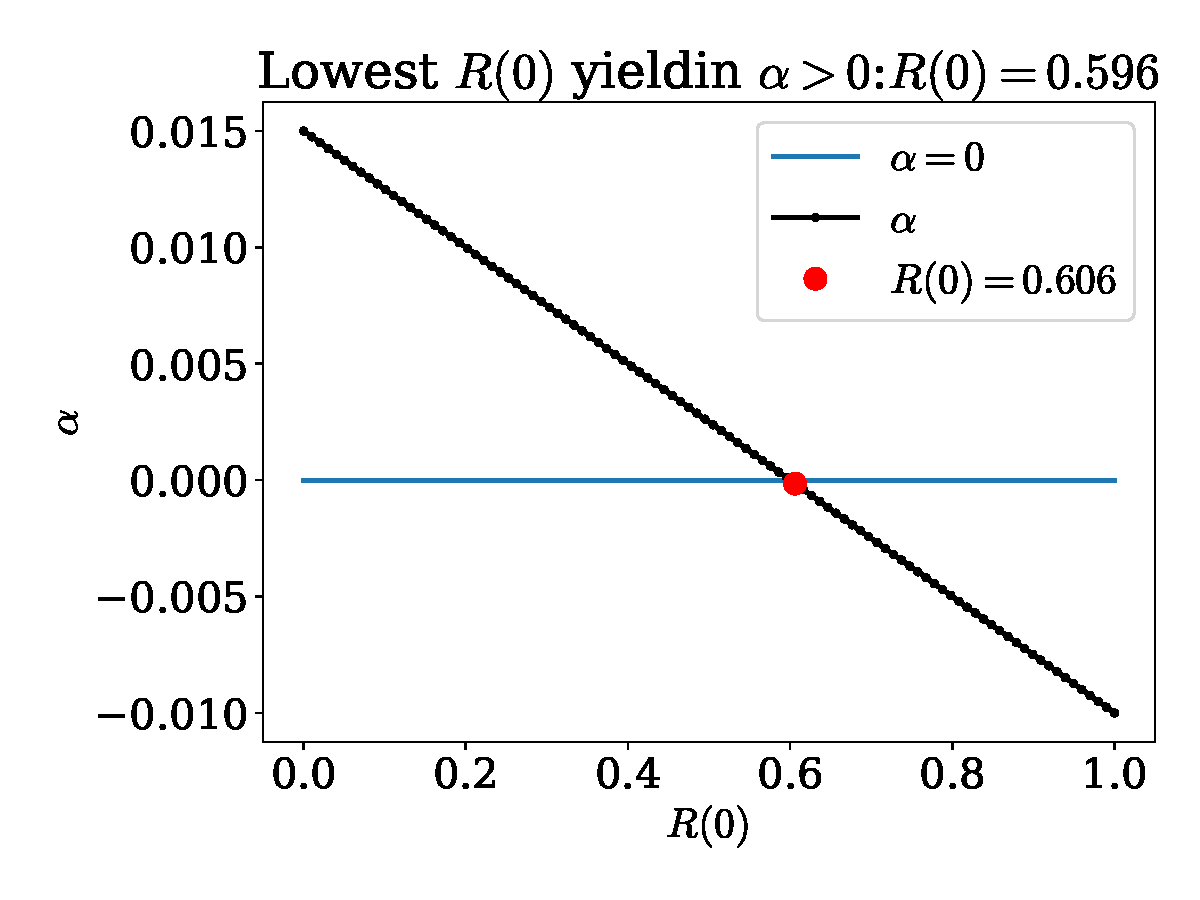
\includegraphics[width=.49\textwidth]{../plots/2A/vax.pdf}
        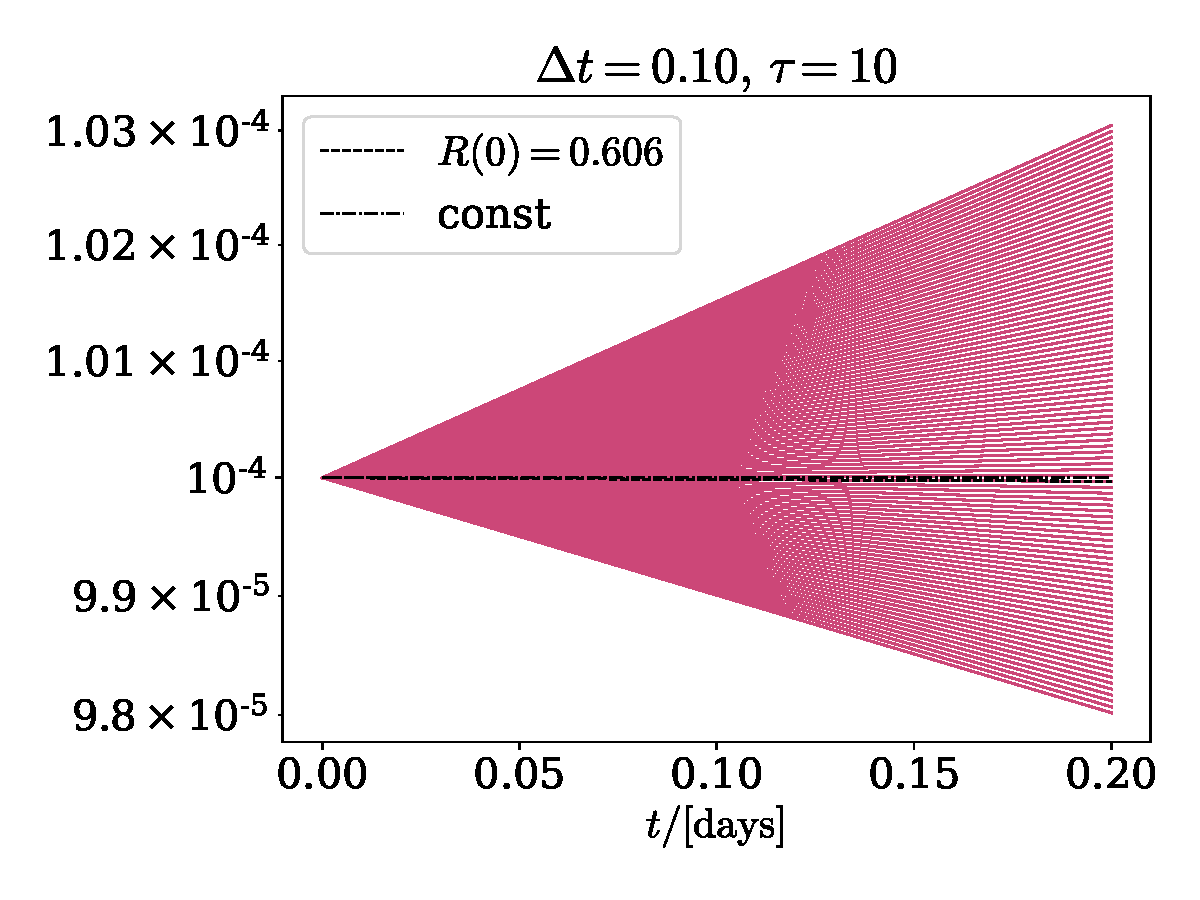
\includegraphics[width=.49\textwidth]{../plots/2A/vax_R.pdf}
        \caption{The plot on the left shows the maximu $R(0)$, i.e. fraction of vaccinated, that still gives exponential growth. The right shows a log-plot of the growht of infected at the very begining.}
        \label{vax}
    \end{figure}

    \subsection*{Stochastic SIR model}
    Next, the stochastic version of SIR model is used. \autoref{stochastic SIR} shows the result of 100 runs, which all give result close to that of the deterministic one. 
    All simulation uses a population of 100\,000, but the plots are normalized. 
    Due to the stochastic nature of the simulation, there is a difference in exactly when the spread takes of. 
    however, as the figure on the right shows, when it does, it grows exponentially at the same rate as the deterministic model. 
    This is also the reason for the spread of the runs around the dashed line in the figure on the right.
    The early days of the infection is susceptible to fluctuations.
    We also see the stochastic model tend to be later than the deterministic.
    (THIS MIGHT HAVE SOMETHING TO DO WITH THE INITIAL CONDITIONS).
    These simulation have been used with $\Delta t = 0.1$ for the stochastic model. 
    \autoref{conv} is a plots the relative error of the simulation, measured as 
    \begin{equation*}
        \Delta R_i = \frac{|R_i(t_0) - R_{\mathrm{ref}}(t_0)|}{R_{\mathrm{ref}(t_0)}},
    \end{equation*}
    where $R_{\mathrm{ref}}$ is some reference value obtained by a simulation with a short step length, and $R_i$ is the value from the simulation with step length $\Delta t_i$.
    The difference is taken at some time $t_0$, which is chosen so that $t_0/\Delta t_i$ is an integer for the time steps in question.
    The values are gotten by taking an average of 100 runs for each value of $\Delta t$
    This result justifies the use of $\Delta t = 0.1$, as it leads to quick simulations, while resulting in errors around $0.02\%$
    Furthermore, the results imply that the method converges as $\Delta t^1$, which means that large gains in precision will be costly.
    
    The stochastic nature of this model makes it possible for the infection to die out, even with $\mathcal{R}_0>1$, by pure chance. 
    \autoref{Disappear} shows a probability for the infection terminating without spreading through the population, for different number of initially infected $I(0)$.
    This data is obtained by running the simulation 1\,000 for each initial condition, and terminating when it either reach $100$ infected, or $0$.
    $100$ infected is observed to yield very high probability of the disease spreading exponentially, and is thus used as a proxy for this.
    This assumption is backed up by the result shown in the figure, where the probability for the infection stopping early is negligible already at $I=10$. 
    $I=0$ means that the infection will no longer spread, and if it does so without ever hitting $I=100$, then the outbreak has disappeared.
    Let $x_i\in\{0, 1\}_{i=1}^n$ be the outcomes of n of the trials, 0 if the outbreaks dies out, 1 if it does not.
    The outcome dying out is then a Bernoulli process, with a probability $p$, which depends on how many are initially exposed.
    The estimator of the probability is then
    \begin{equation*}
        p = \frac{1}{n}\sum_{i=1}^n x_i.
    \end{equation*}
    The unbiased estimator of the variance of the Bernoulli distribution is
    \begin{equation*}
        s^2 = \frac{1}{n} \sum_{i=1}^n (p - x_i)^2.
    \end{equation*}
    This is not a measure of the error in it self, but rather a estimation of a parameter of the underlying distribution. 
    The standard error, $\sqrt{s^2/n}$, gives a estimation of the standard deviation of the sampling distribution, and is therefore used as a measure of the error. \footnote{\url{https://en.wikipedia.org/wiki/Standard_error}}
    \autoref{Disappear} shows the estimation of the probability of the outbreak dying out, together with the uncertainties, from 1000 runs of the simulation for initial value of infected.

    \begin{figure}[H]
        \centering
        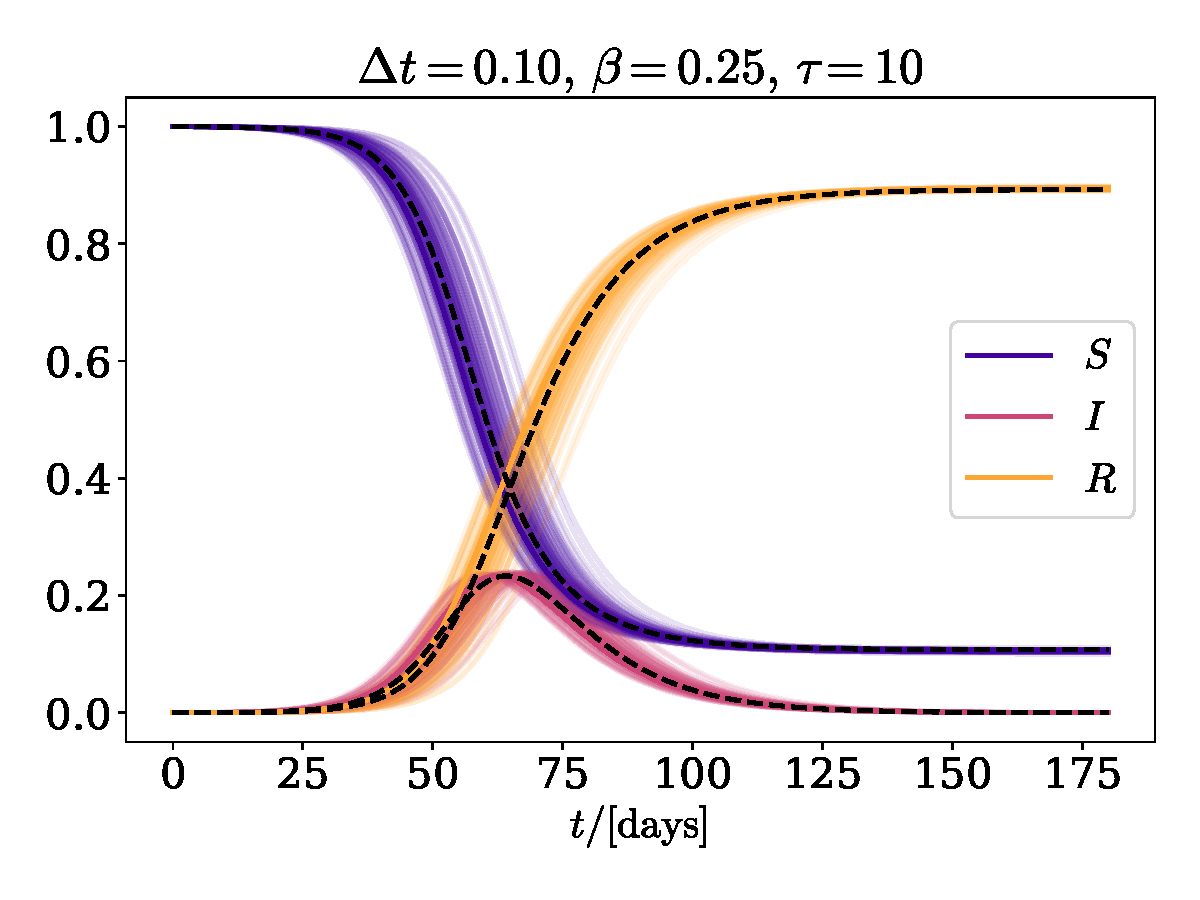
\includegraphics[width=.49\textwidth]{../plots/2B/TestSIR_stoch.pdf}
        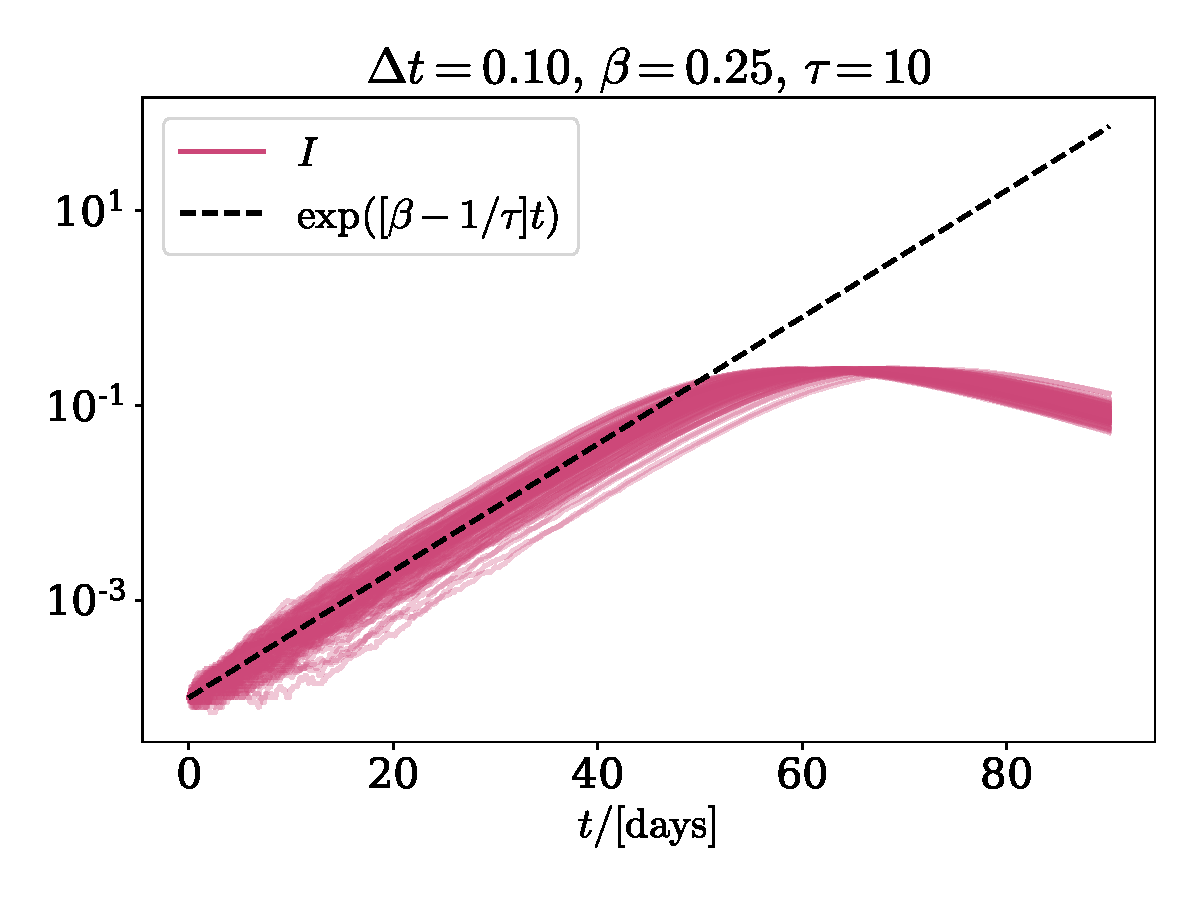
\includegraphics[width=.49\textwidth]{../plots/2B/TestI_stoch.pdf}
        \caption{100 runs of the stochastic SIR model. All runs are close to the deterministic, showed as dashed lines}
        \label{stochastic SIR}
    \end{figure}

    \begin{figure}[H]
        \centering
        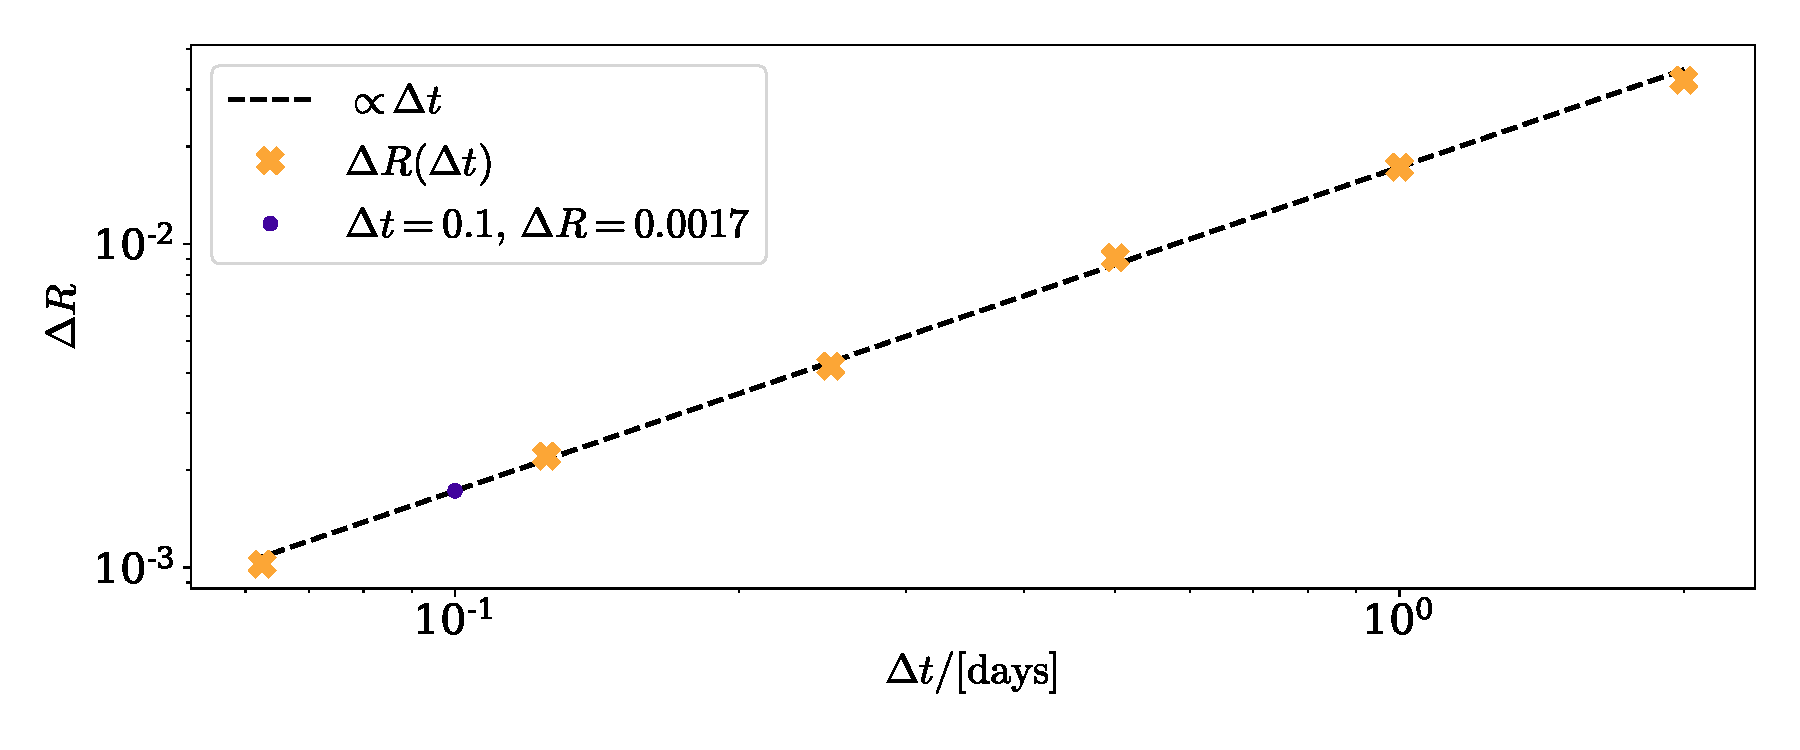
\includegraphics[width=.7\textwidth]{../plots/2B/conv.pdf}
        \caption{The relative eviation of the value of $R$ at $t=200$, for different step lengths $\Delta t$}
        \label{conv}
    \end{figure}


    \begin{figure}[H]
        \centering
        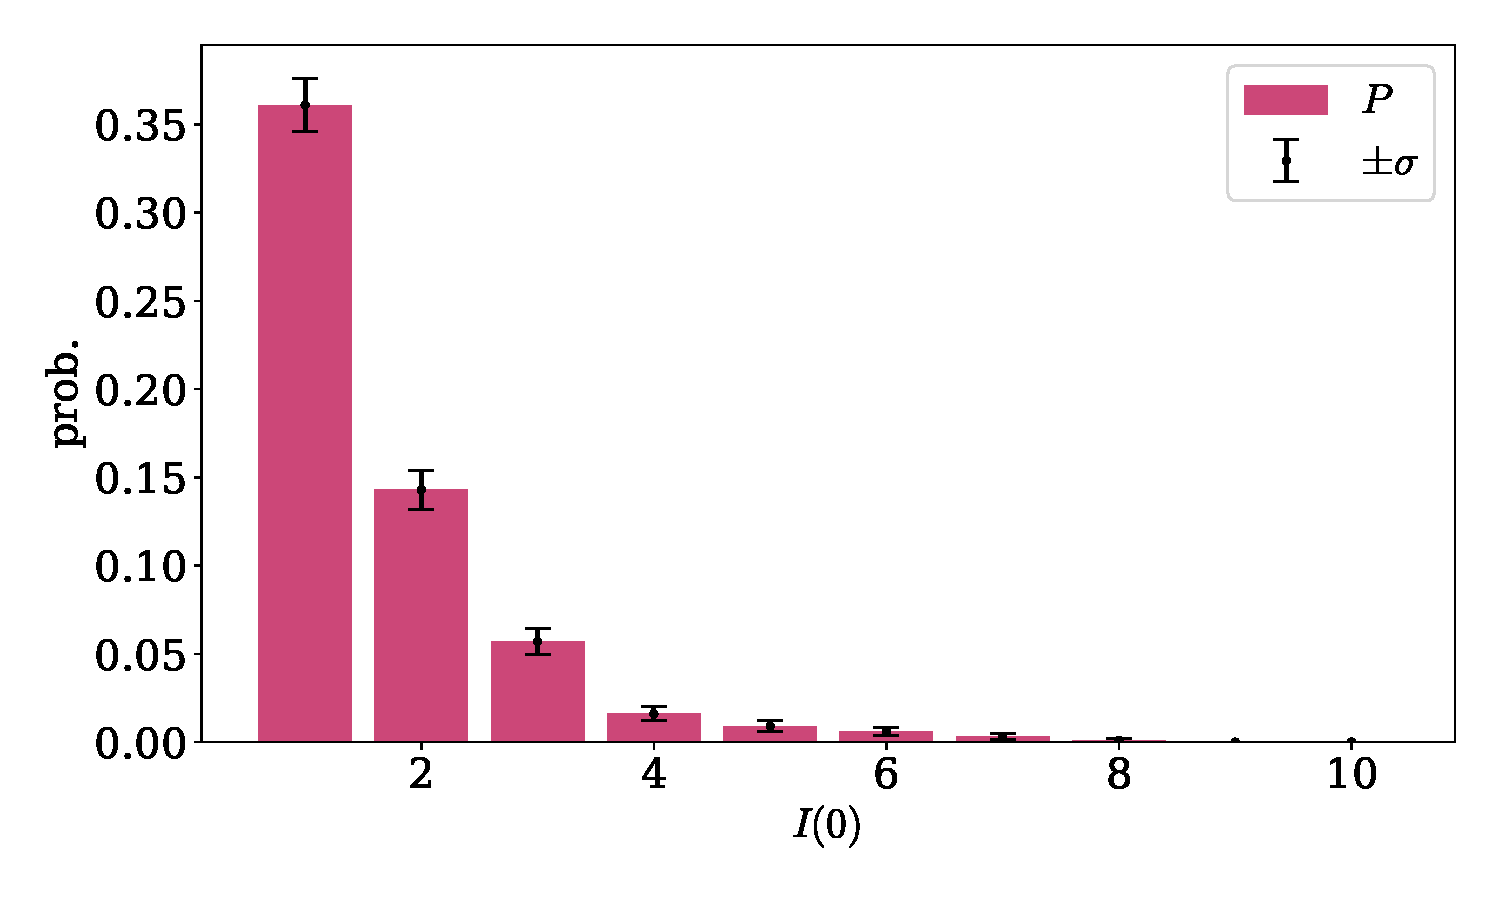
\includegraphics[width=.7\textwidth]{../plots/2B/disappear.pdf}
        \caption{The probability that the infection dies, for different starting values of $I$. Each probability is caculated from an average of 1\,000 runs, while the error bar indicate one standard deviation, obtained from 10 averages of 100 runs.}
        \label{Disappear}
    \end{figure}

    \subsection*{SEIIaR model}
    The SEIIaR model incorporates the possibility of asymptomatic infection, $I_a$, as well as a incubation period, $E$, as well as a set of new parameters, described in \cite{exam}.
    \autoref{SEIIaR} shows 10 runs of the simulation, and compares it to the result from the deterministic SIR model.
    The same asymptotic values are reach for $S$ and $R$, however, due to the incubation period, the raise in infection is delayed somewhat.
    \autoref{SEIIaR conv} show a estimation of the error, where a simulations with different time step is compared to a reference simulation, all averaged over 100 runs.
    This shows that a timestep $\Delta = 0.1$ should still yield high precision.

    Infected people with symptoms, $I$, can self isolate, and thus decrease the spread of the disease.
    This is controlled by the $r_a$ parameter.
    If it is $1$, the symptomatic are as likely to infect others as $\mathcal{R}_0 = \beta \tau $ would suggest. 
    However, if it is less, for example due to isolation, then the spread will subside.
    \autoref{isolation} shows the early evolution of the exposed population, $E$, for $r_s\in [0, 1]$.
    Each line is an average of 100 runs.
    Due to this population not being infectious, it will initially decrease.
    The measure of the exponential increase is therefore taken as $\alpha = \ln\left(E(20)/E(5)\right)/(15 \mathrm{days})$.
    The largest $r_s$ that do not result in exponential growth is $r_s = 0.40$
    
    \begin{figure}[H]
        \centering
        \begin{subfigure}{.49\textwidth}
            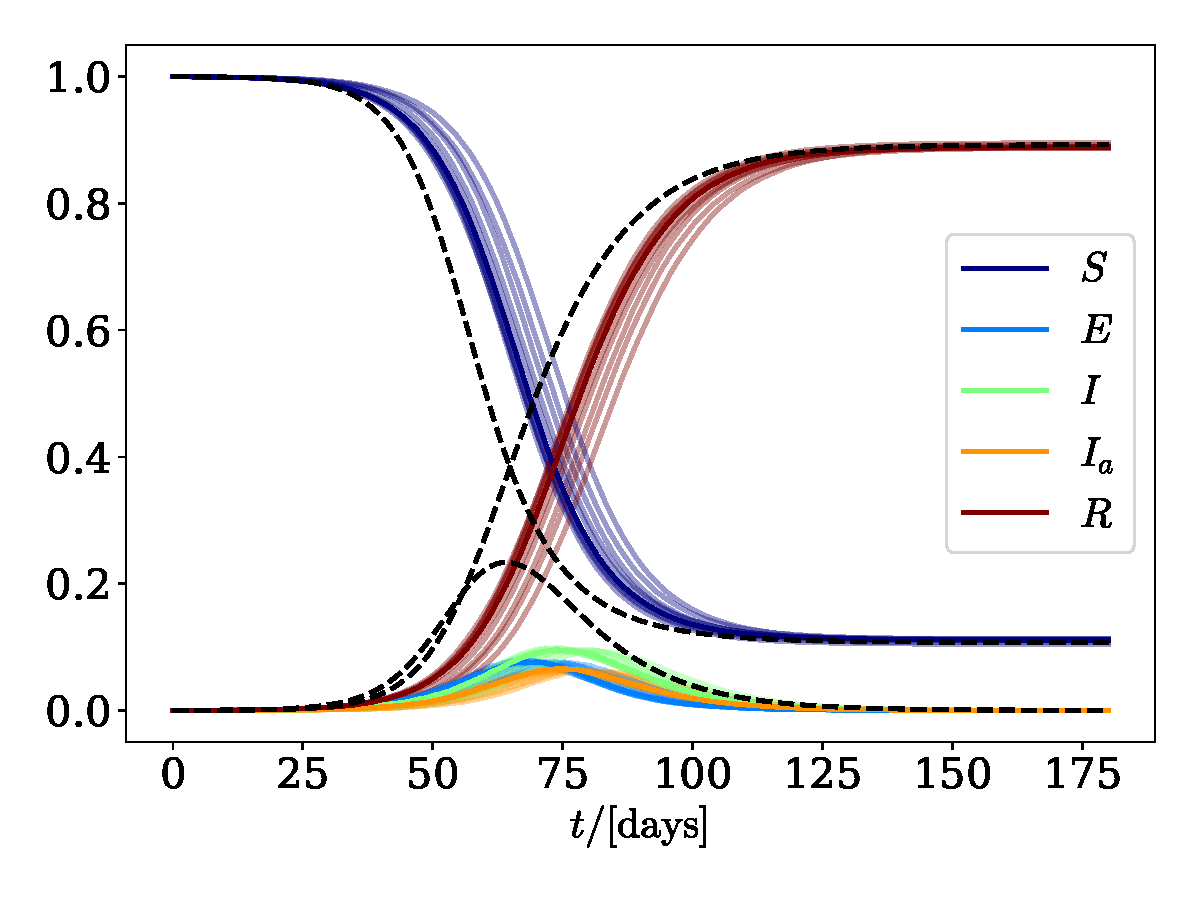
\includegraphics[width=\textwidth]{../plots/2C/TestSEIIaR.pdf}
            \caption{10 runs of the SEIIaR model.}
            \label{SEIIaR}
        \end{subfigure}
        \begin{subfigure}{.49\textwidth}
            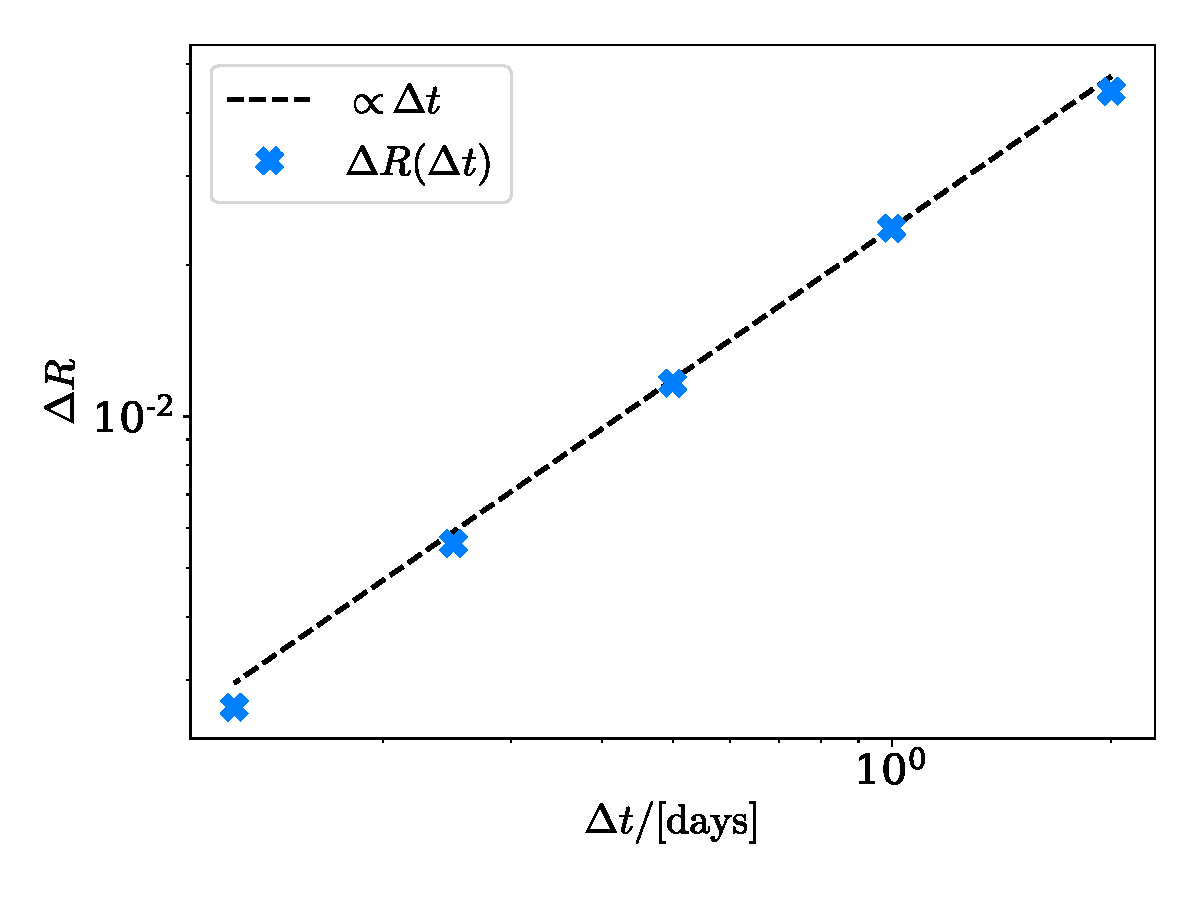
\includegraphics[width=\textwidth]{../plots/2C/conv.pdf}
            \caption{Error relative a reference run of the SEIIaR model.}
            \label{SEIIaR conv}
        \end{subfigure}
    \end{figure}

    \begin{figure}[H]
        \centering
        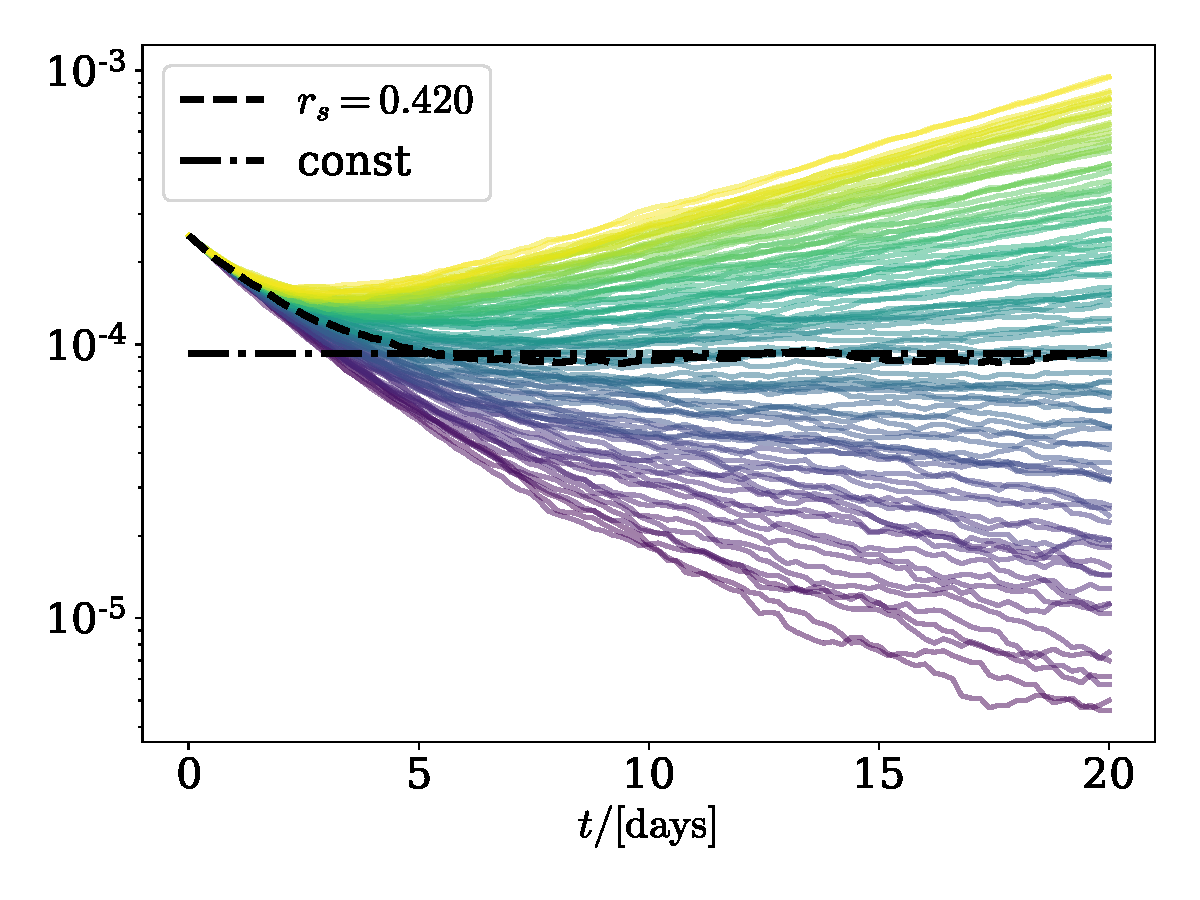
\includegraphics[width=.7\textwidth]{../plots/2C/isolation.pdf}
        \caption{cap}
        \label{isolation}
    \end{figure}


    \subsection*{SEIIaR commuter model}
    The last complication of the model is to include the fact that people live and work at different places, and might bring with them the infection when commuting. 
    The traveling pattern of the population is encoded in a matrix, as described in \cite{exam}.
    Given a matrix without off diagonal elements, each city should have evolve exactly as they do in the non-commuter SEIIaR test.
    This is thus a good check on the implementation.
    \autoref{SEIIaR commute} shows the result in one of the cities of such a run in.
    This city did not have any commuters, and the same initial conditions, and should therefore yield identical results, modulo the inherit randomness of the, which a comparison with \autoref{SEIIaR} confirms.
    Furthermore, the error showed in \autoref{SEIIaR commute conv} behaves as the non-commuter model
    Another test for the commuter model is to let the entire population be commuters, i.e. only off-diagonal elements are non zero, and start with infections only in one of these populations.
    Then, the spread should be contained to this population.
    This case is illustrated in \autoref{All commuters}, confirming that the model behaves as expected.

    Next, the system described by the matrix in Equation 10 in \cite{exam} is simulated.
    The result in each town is showed in \autoref{two towns}
    (ADD MORE DATA: WHEN DO THEY PEAK; WHAT ARE THE ASYMPTOTES. DISCUSS)
    Next, a system with 10 towns is simulated. 
    In this system, there are two large towns, town 1 and 5, and eight smaller towns, in groups of four which are connected to one of of the large towns.
    \autoref{nine towns} shows the evolution of the infection.
    The infection starts in town 2, which explains why it is the first to reach the peak of the infection, at day 57.
    It then spreads to town 1, as it is a hub connected to town 2, which has the peak of its infection at day 103. 
    Town 3, 4 and 4, all satellites of town 1 all hit their peak around day 120.
    The infection then spreads to the other hub, town 6, as it is connected to town 1, which has its peak at day 145, before it at last spreads to the satellites of town 6, town 7, 8, 9 and 10, which all have their peak around day 160.

    \begin{figure}[H]
        \centering
        \begin{subfigure}{.49\textwidth}
            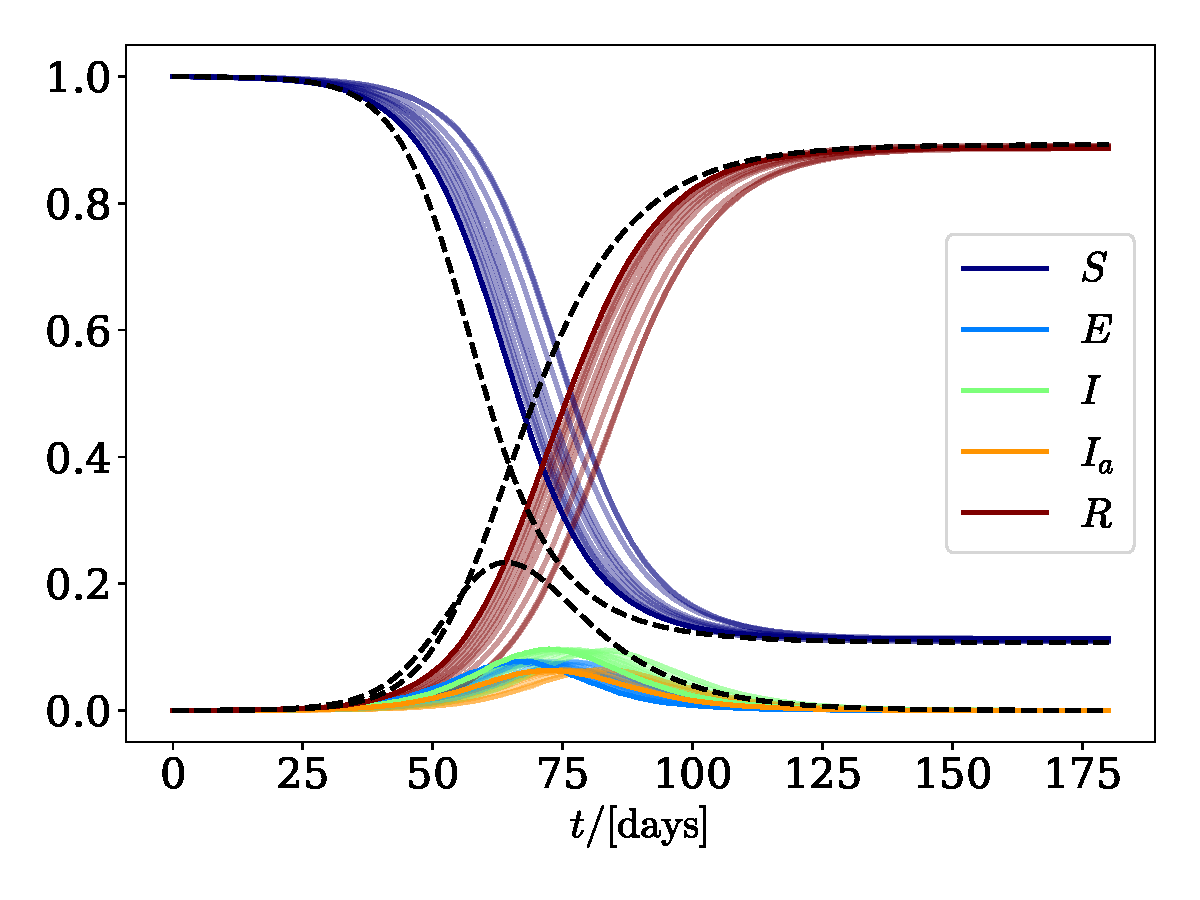
\includegraphics[width=\textwidth]{../plots/2D/TestSEIIaR_commute.pdf}
            \caption{10 runs of the SEIIaR commuter model.}
            \label{SEIIaR commute}
        \end{subfigure}
        \begin{subfigure}{.49\textwidth}
            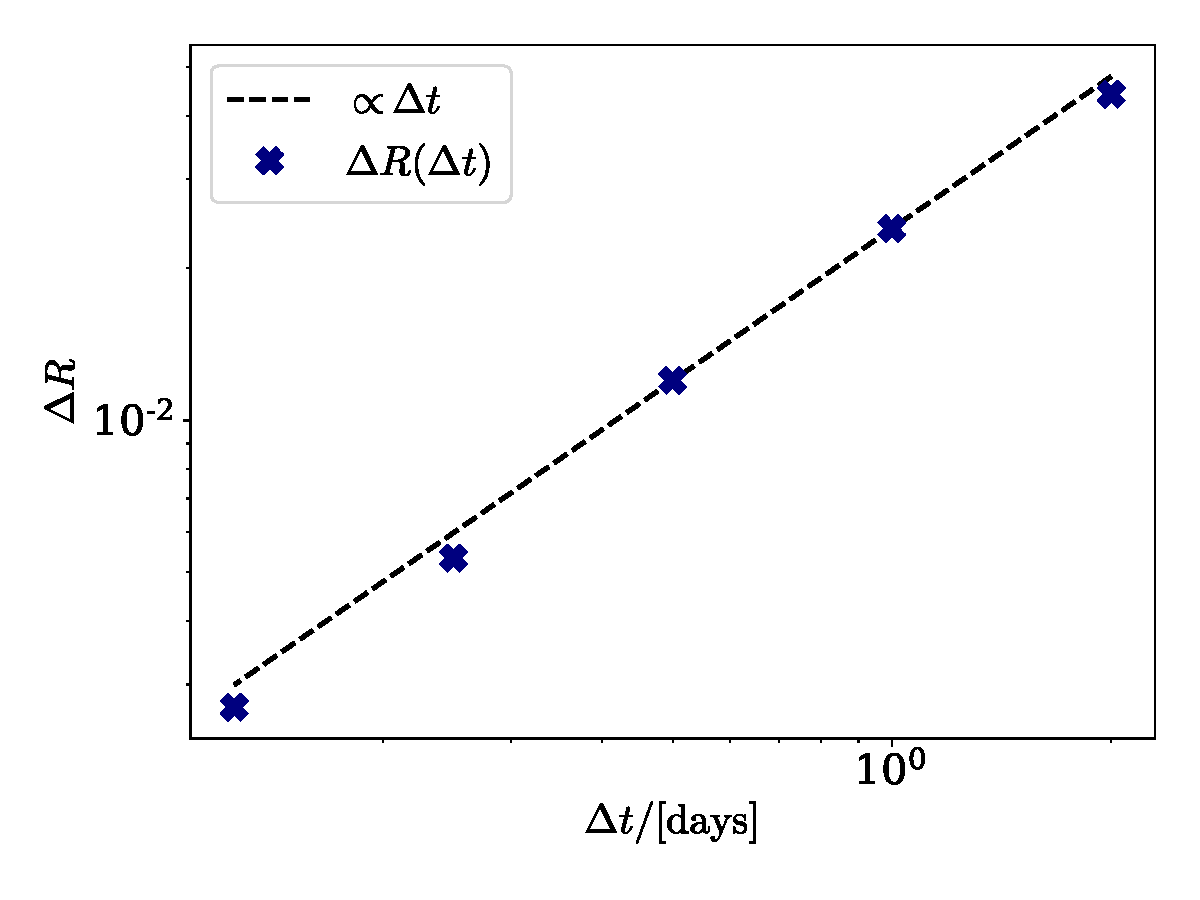
\includegraphics[width=\textwidth]{../plots/2D/conv.pdf}
            \caption{Two towns, where everyone commutes, and the infection is only present in one of them at the start. }
            \label{SEIIaR commute conv}
        \end{subfigure}
    \end{figure}

    \begin{figure}[H]
        \centering
        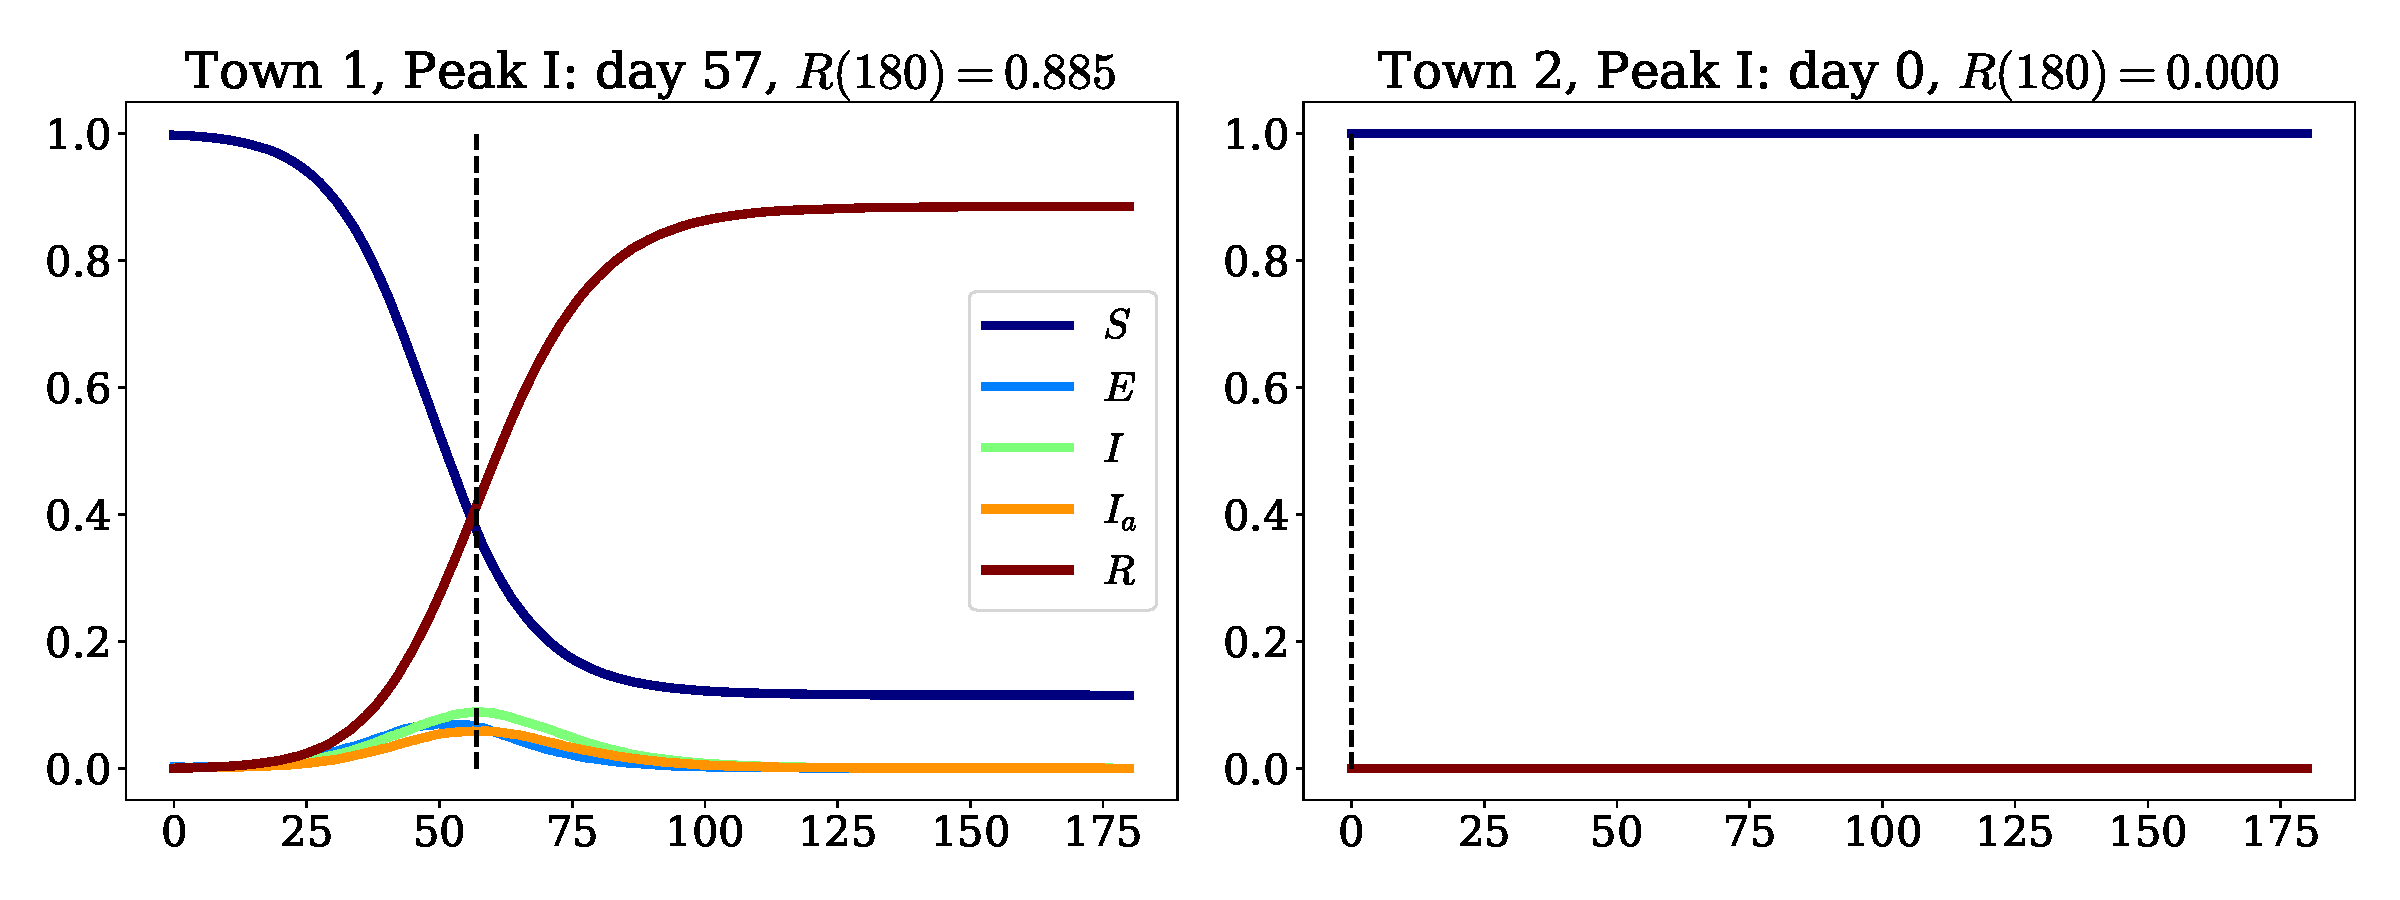
\includegraphics[width=.7\textwidth]{../plots/2D/two_towns2.pdf}
        \caption{Two towns, where everyone commutes, and the inital infection is only present in one of them. The plots shows that the infection is contained, as expected.}
        \label{All commuters}
    \end{figure}

    \begin{figure}[H]
        \centering
        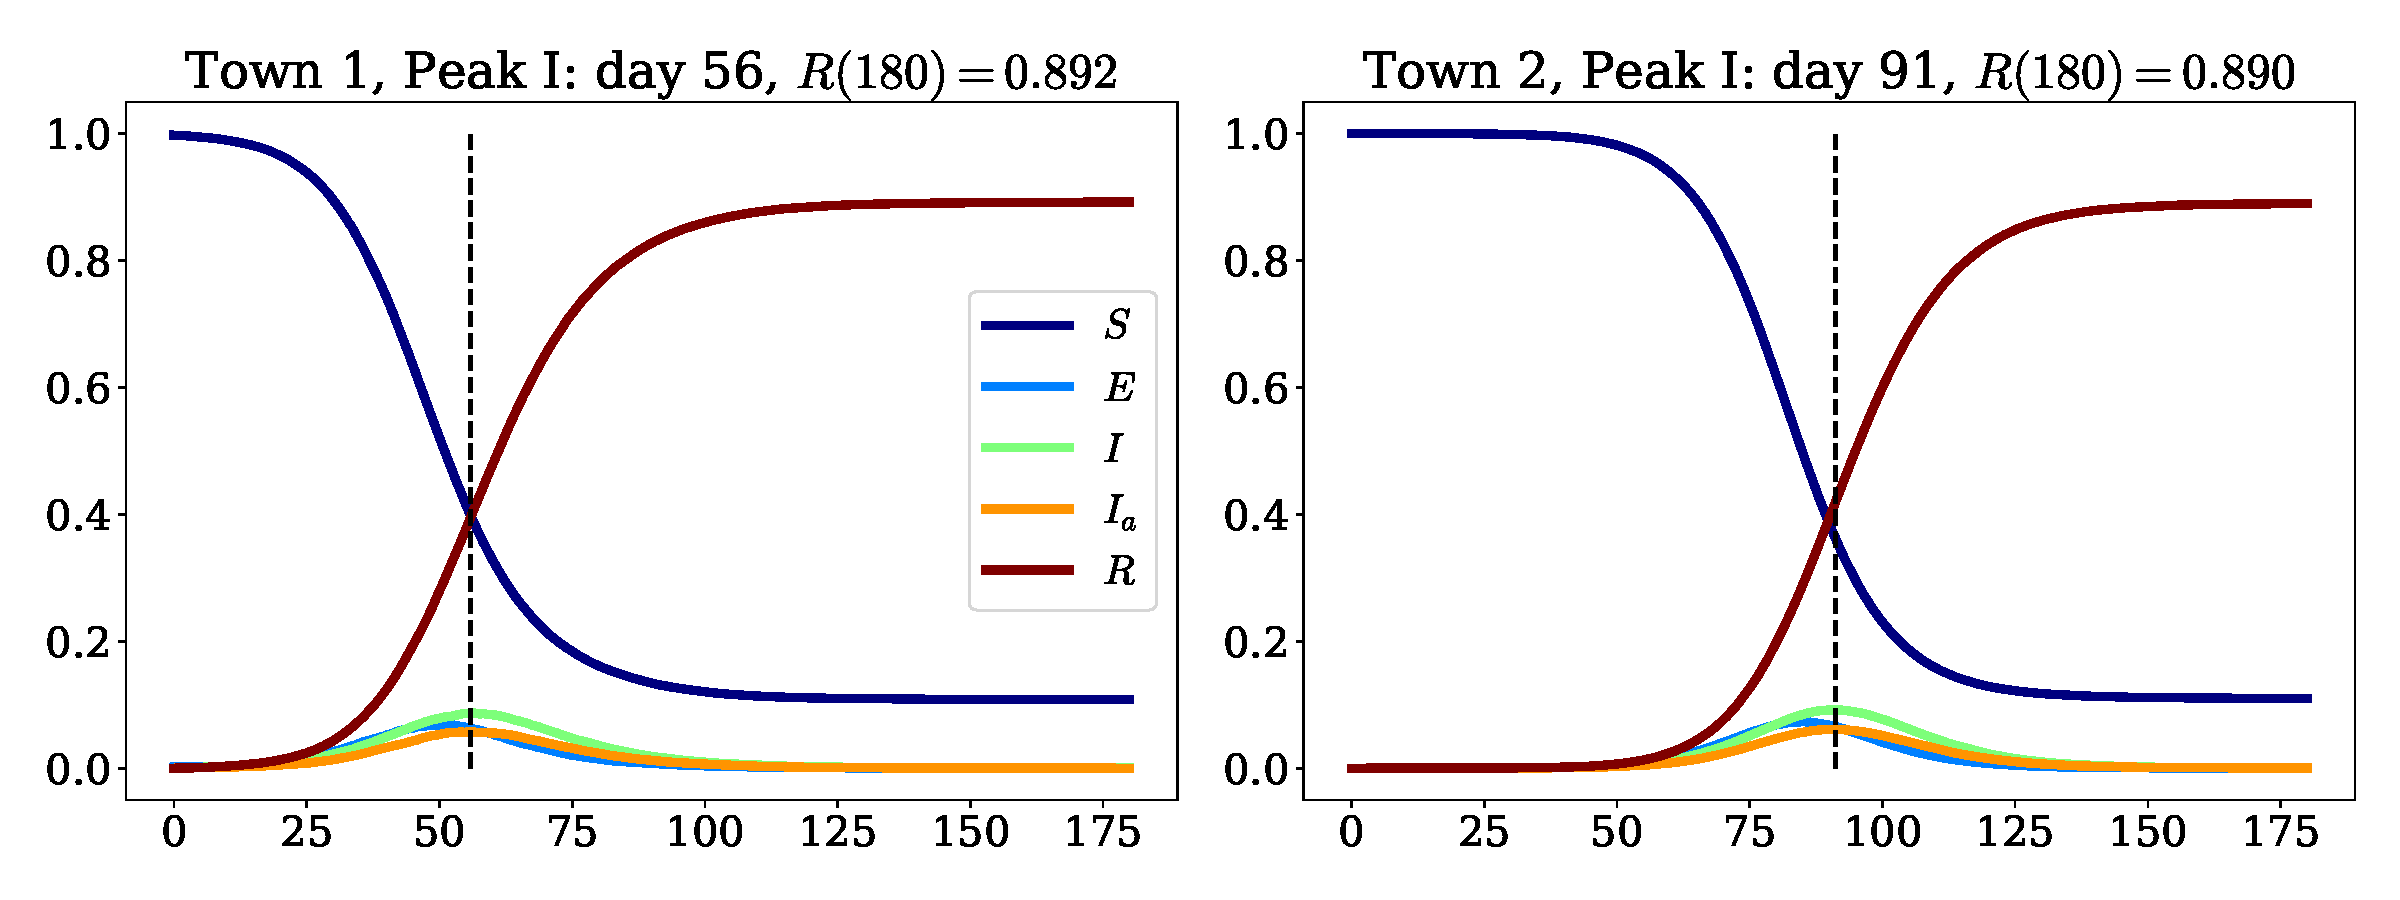
\includegraphics[width=.7\textwidth]{../plots/2D/two_towns.pdf}
        \caption{Spread of the infections in two connected towns. The lines are averages of 10 runs.}
        \label{two towns}
    \end{figure}

    \begin{figure}[H]
        \centering
        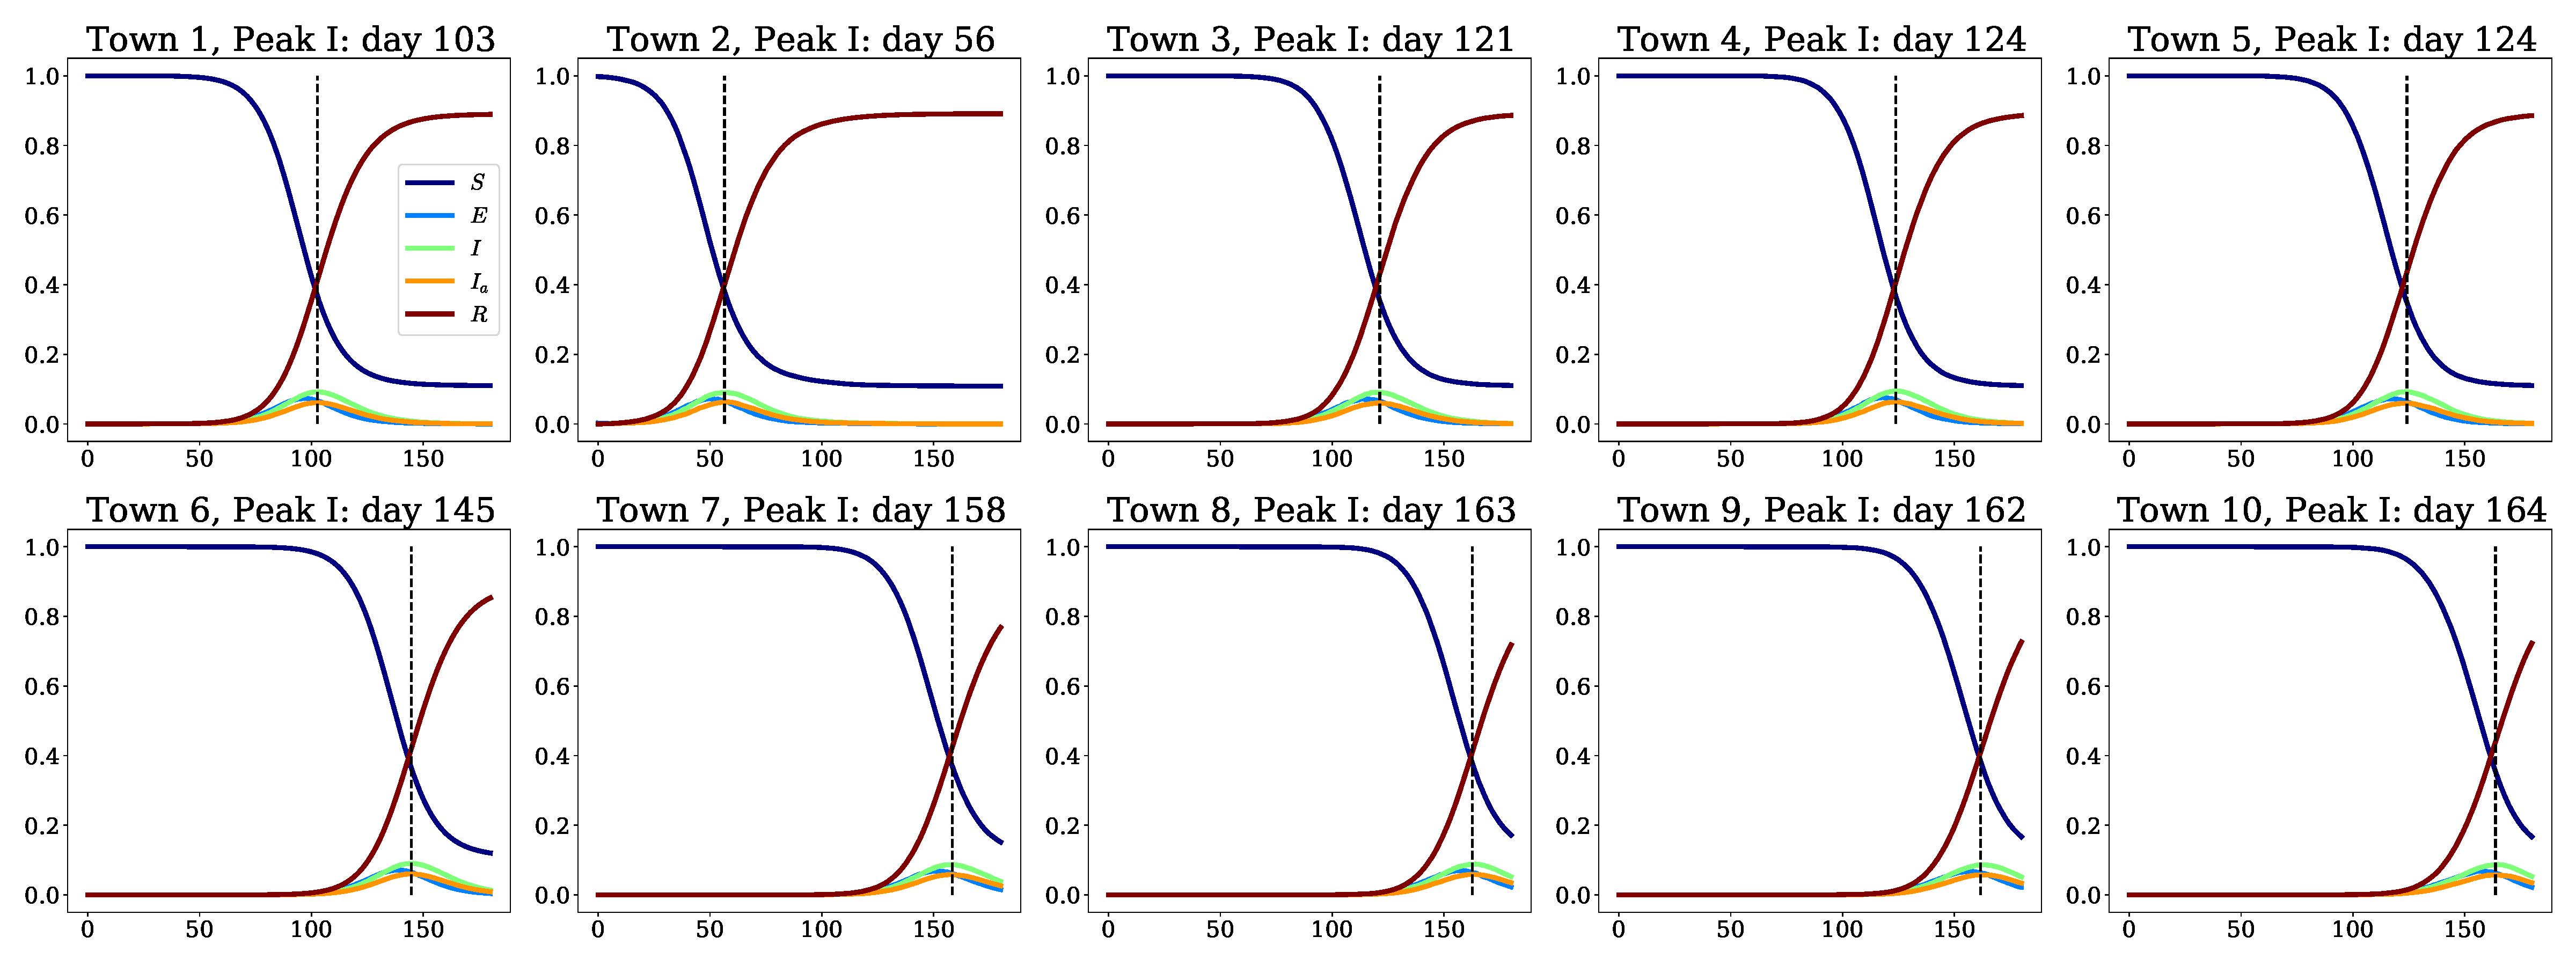
\includegraphics[width=\textwidth]{../plots/2D/nine_towns.pdf}
        \caption{The evloution of the infection in 10 connected towns.}
        \label{nine towns}
    \end{figure}

    The last system to be simulated is a model of Norway, with the working populace of Norway spread throughout 356 cities and towns. 
    The system is represented in a $356 \times 356$ matrix with $356 \cdot 355 /2 = 63190$ different populations, many of which are zero.
    The simulation will be used to investigate the effects of reducing travel.
    This is done by cutting the off diagonal elements of the population matrix, representing those who travel to a different town for work, by 90\%, and increasing the population in their corresponding home town to keep the population living in that city constant.
    \autoref{pop structure} illustrates the population matrix before and after the lockdown, as well as the population distribution of towns in question.
    The effect to be investigated is how lockdown changes how many towns have an outbreak at once.
    An outbreak is defined as more than a total of 10 people infected, where we count both symptomatic and and asymptomatic infections i.e. $I_\mathrm{tot}=I + I_a$.
    The simulation is run by starting with $E=50$ in town 1, Oslo, then taking the average of 10 runs for both population matrices.
    \autoref{towns infected} shows the evolution of the infection, in both cases. 
    On the left is the case without any restriction, and on the right is the case where commuting is reduced by 90\%. 
    This shows that the lockdown somewhat slows the spread.
    In the case of no lockdown, there is a period where all towns have a active infection, while the slows the spread down, resulting in a lower peak.
    \autoref{Oslo Bergen} compares the spread in the largest and second largest city, with and without lockdown.
    The largest town, town 1, is more or less unaffected, as it is where the spread started.
    The second largest town, town 237, is however affected.
    The peak in this town is delayed by around a month due to the lockdown.


    \begin{figure}[H]
        \centering
        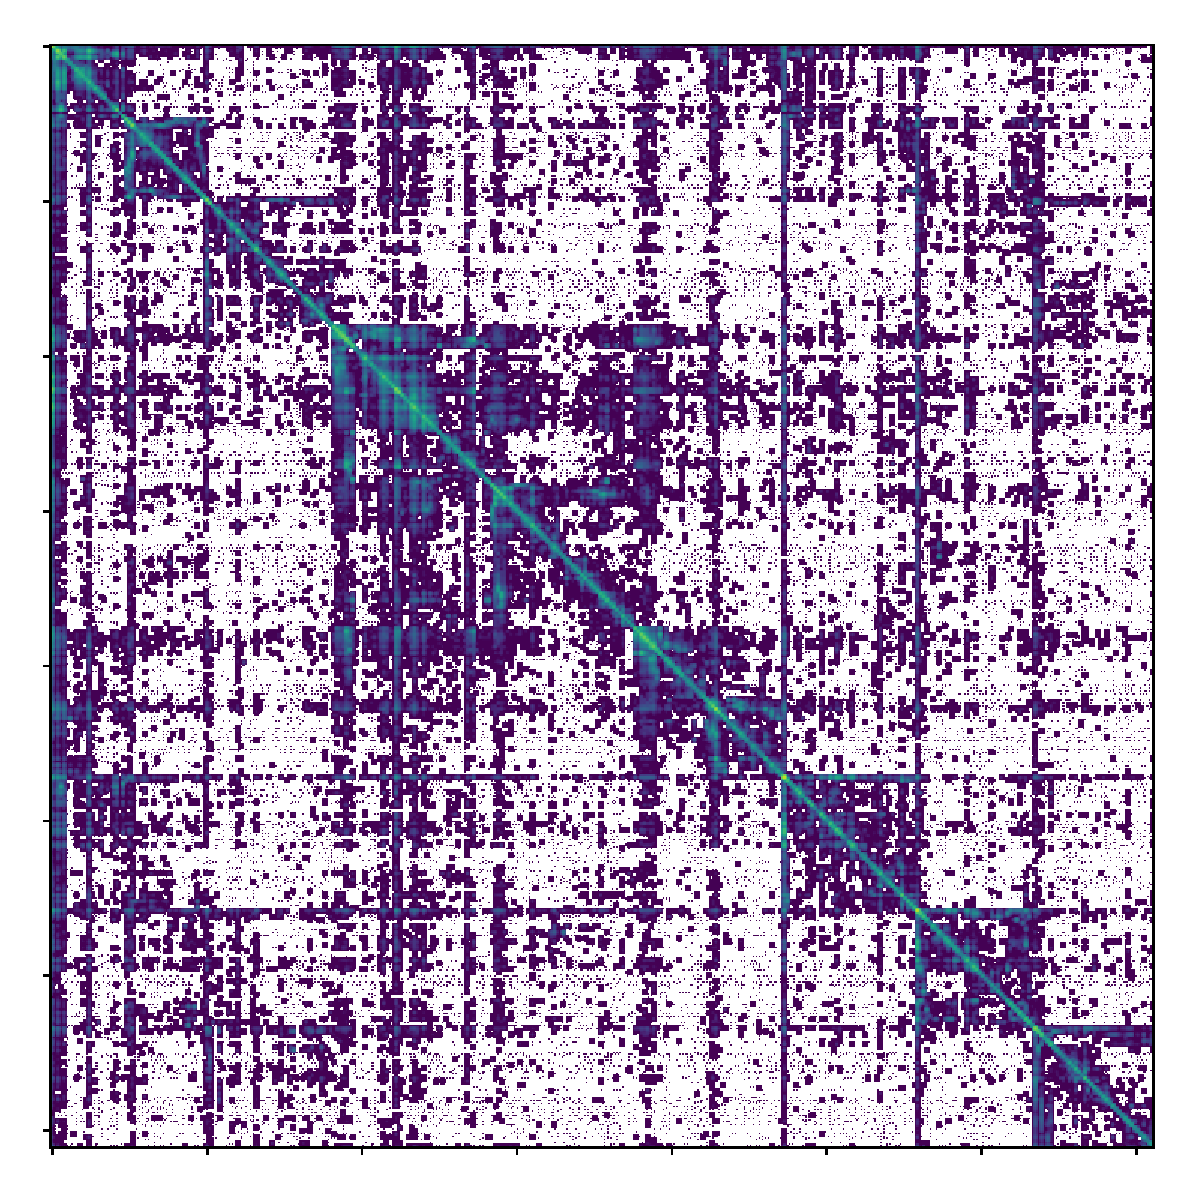
\includegraphics[width=.30\textwidth]{../plots/2D/pop_struct.pdf}
        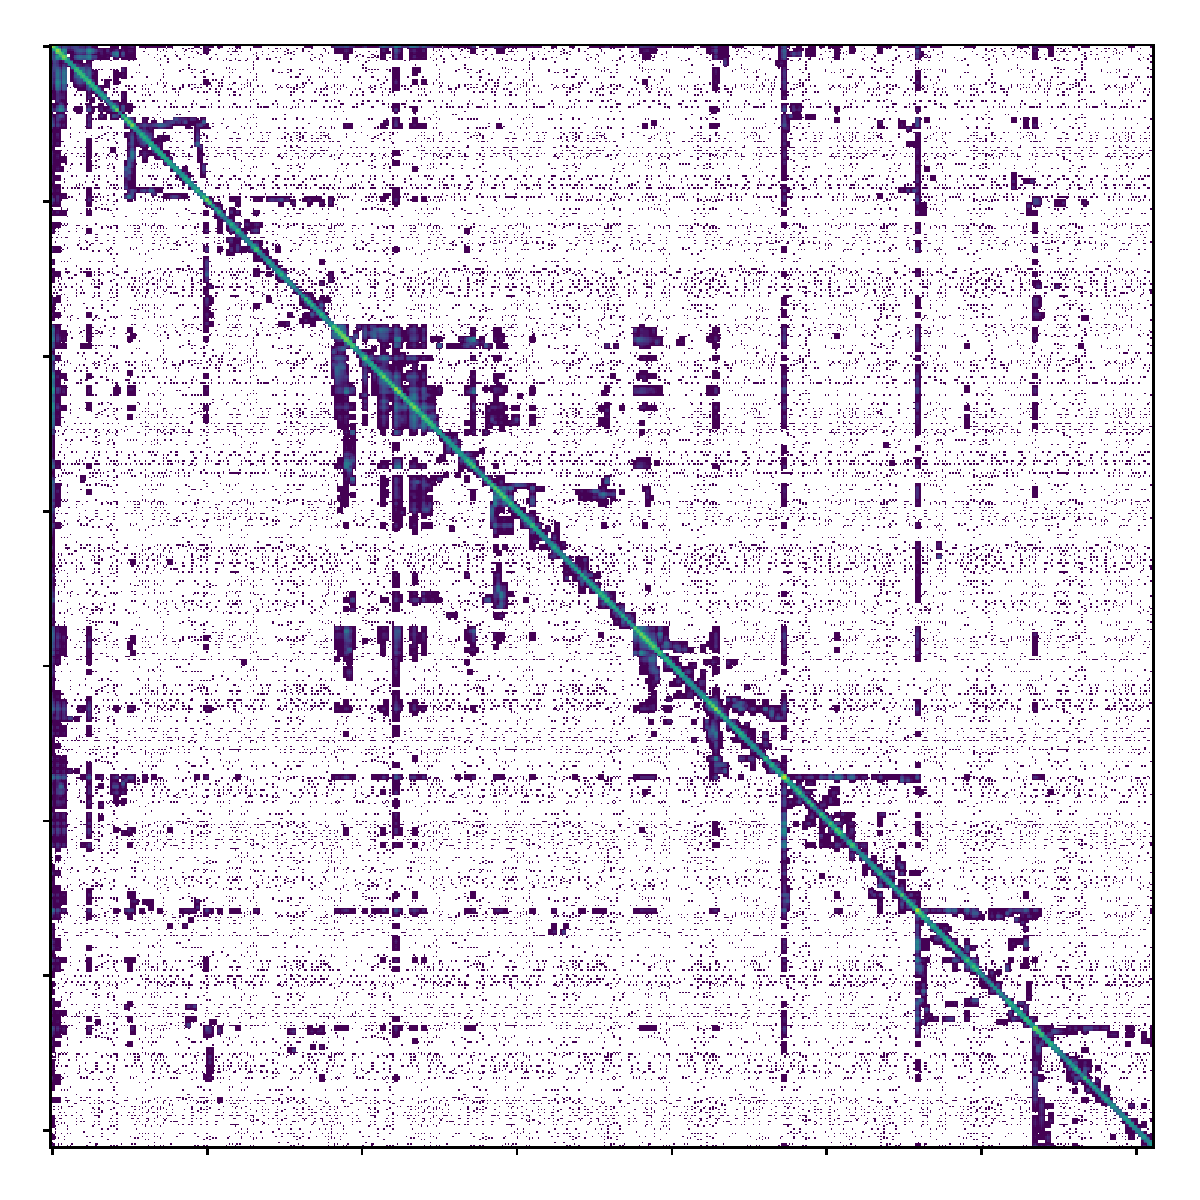
\includegraphics[width=.30\textwidth]{../plots/2D/pop_struct_lockdown.pdf}
        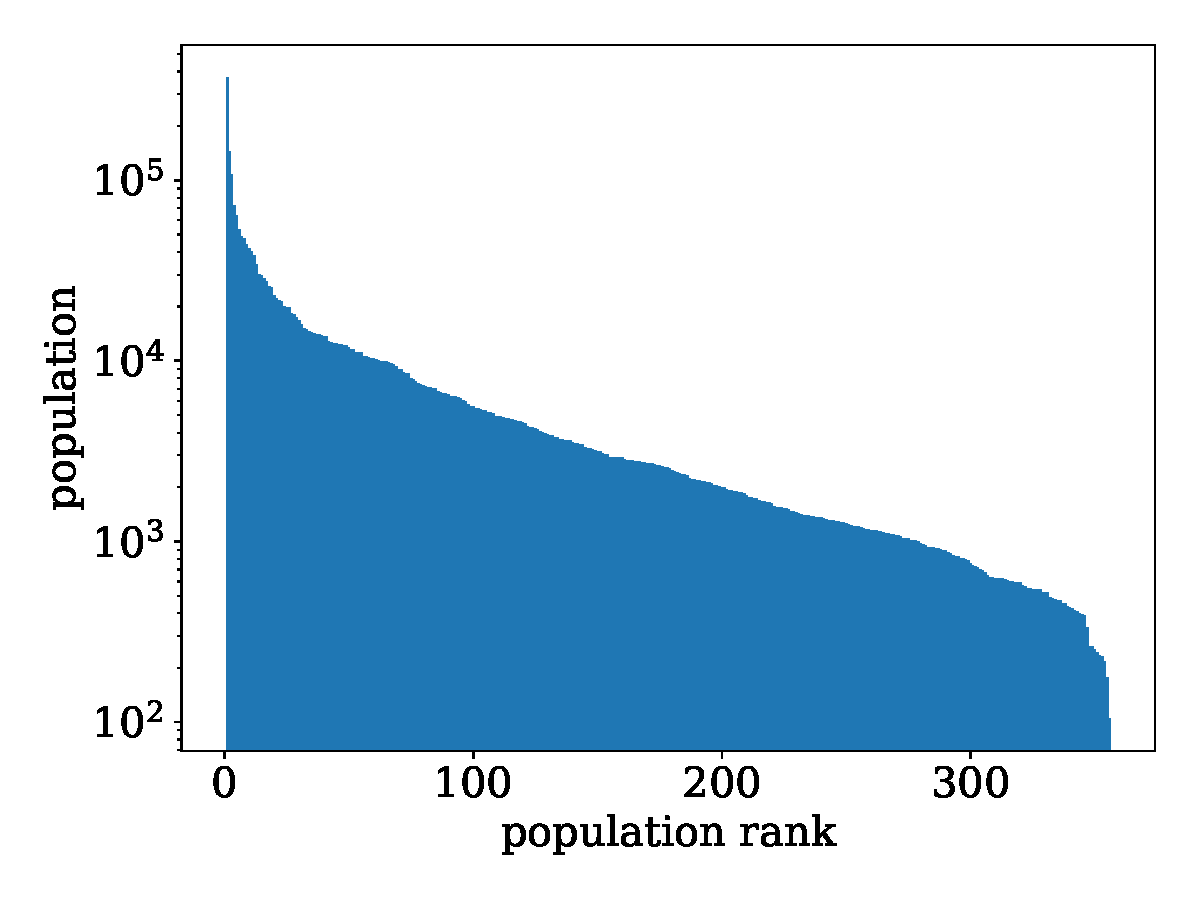
\includegraphics[width=.38\textwidth]{../plots/2D/pops.pdf}
        \caption{cap}
        \label{pop structure}
    \end{figure}

    \begin{figure}[H]
        \centering
        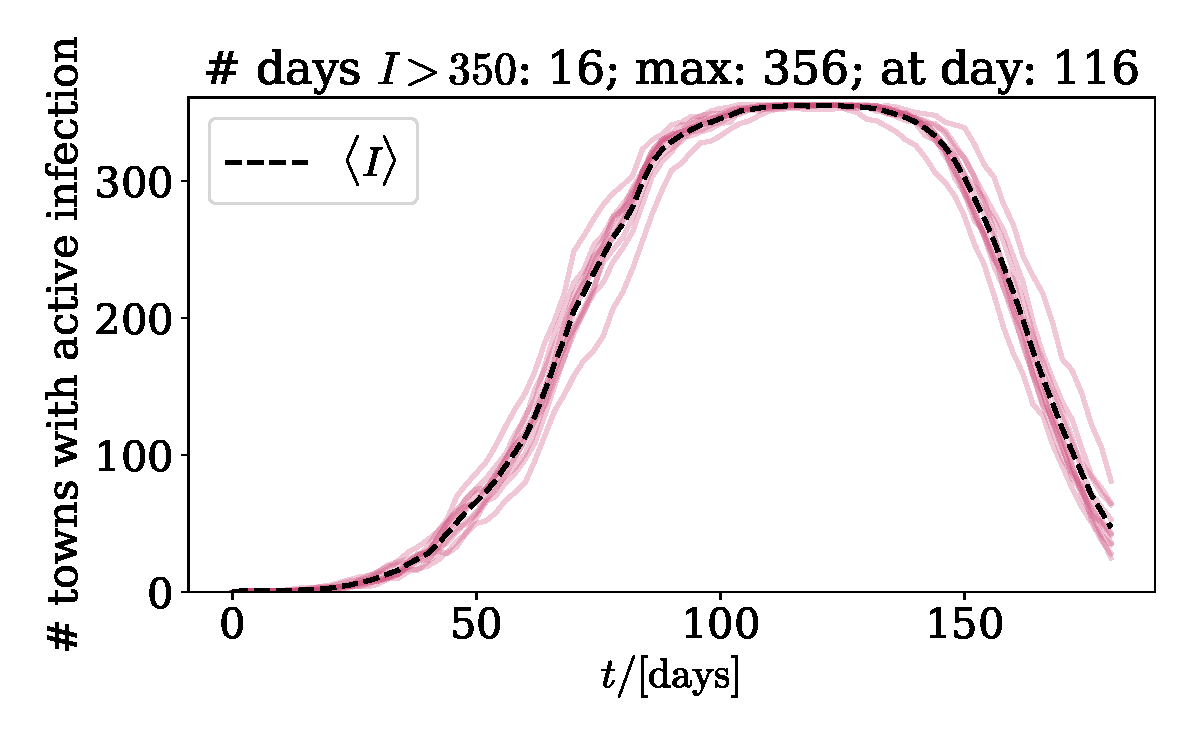
\includegraphics[width=.49\textwidth]{../plots/2D/num_infected.pdf}
        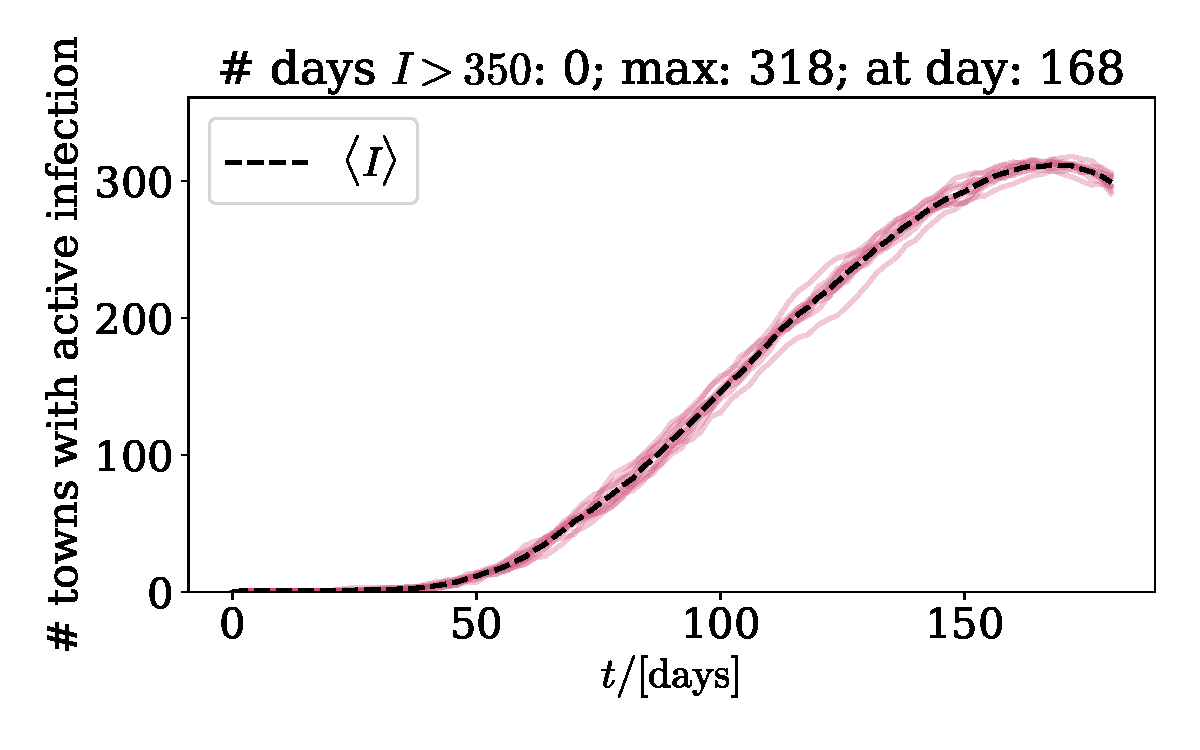
\includegraphics[width=.49\textwidth]{../plots/2D/num_infectedlockdown.pdf}
        \caption{cap}
        \label{towns infected}
    \end{figure}

    \begin{figure}[H]
        \centering
        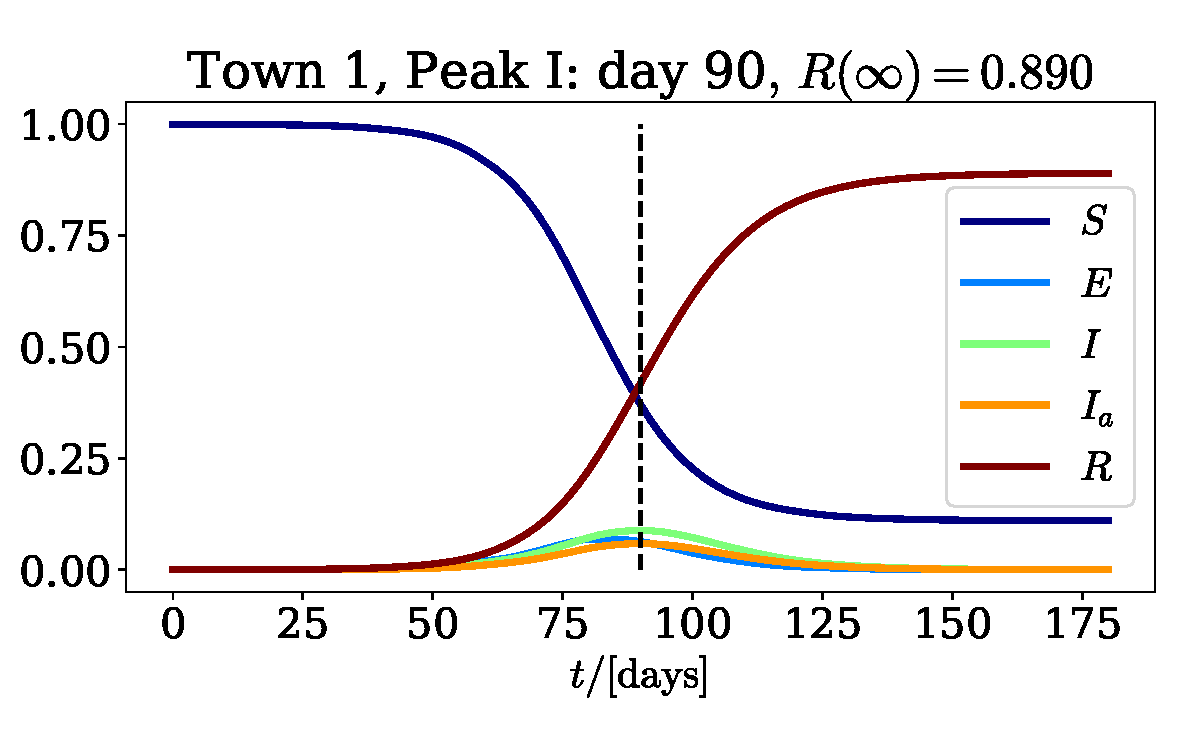
\includegraphics[width=.49\textwidth]{../plots/2D/Oslo.pdf}
        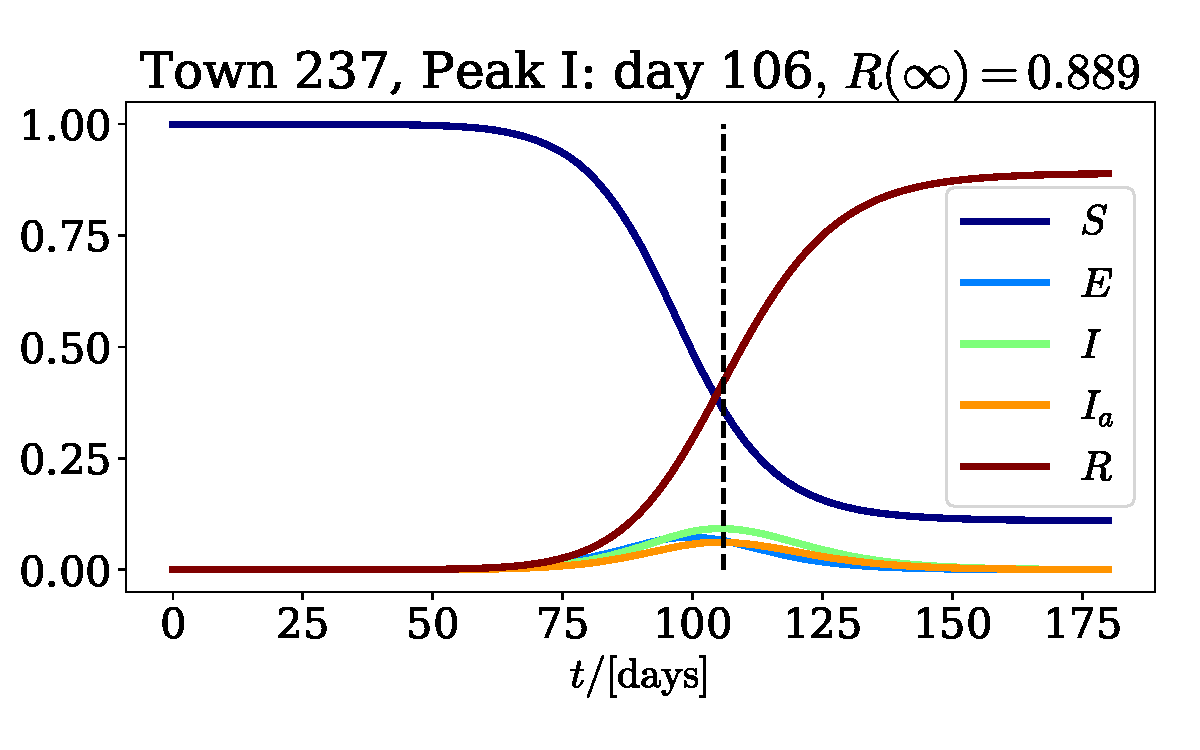
\includegraphics[width=.49\textwidth]{../plots/2D/Bergen.pdf}
        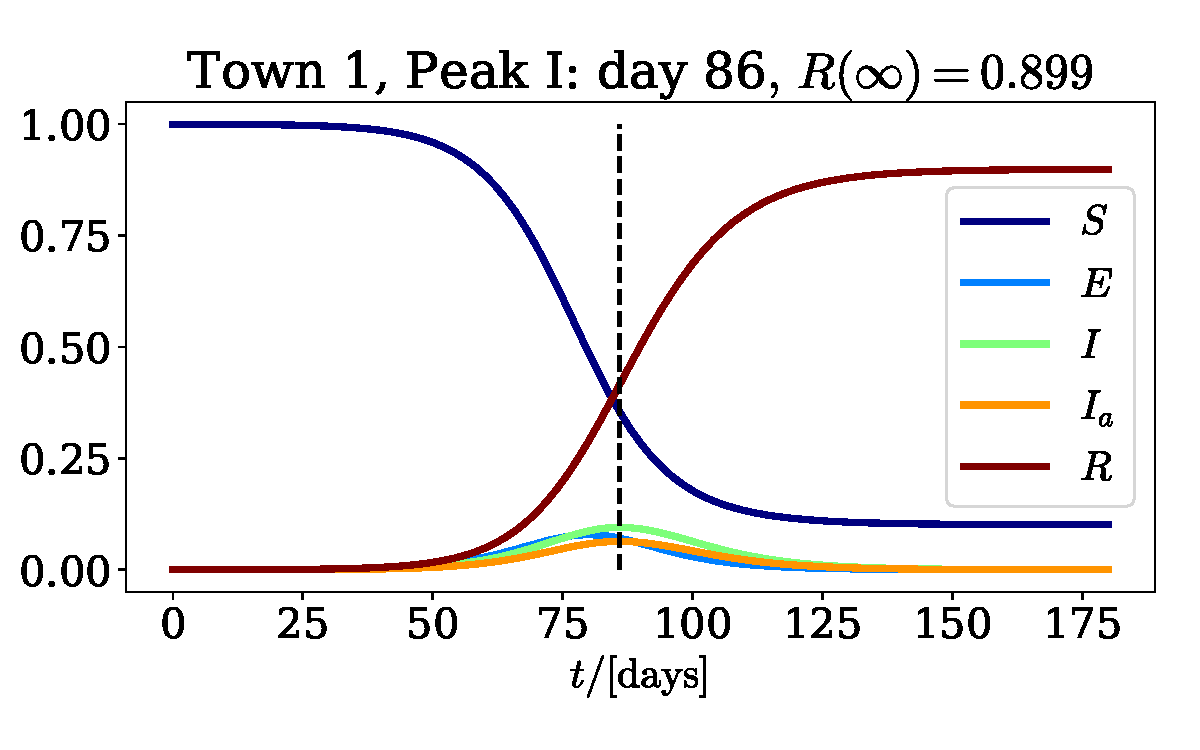
\includegraphics[width=.49\textwidth]{../plots/2D/Oslolockdown.pdf}
        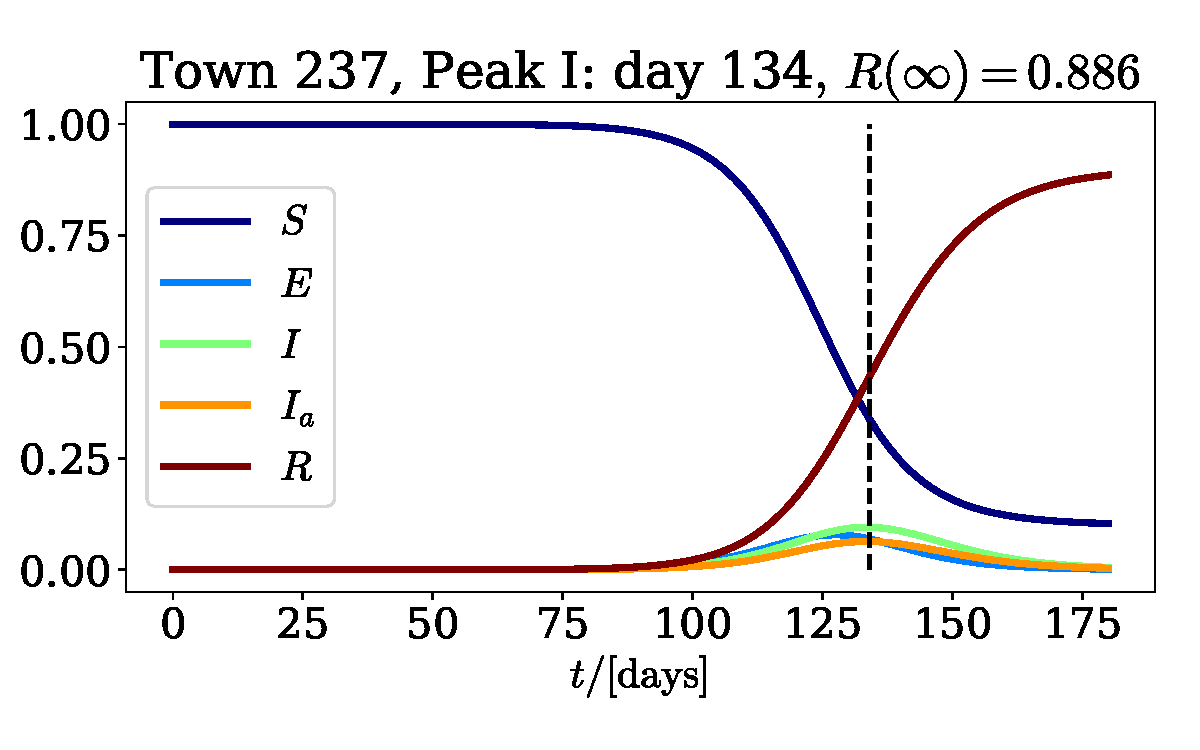
\includegraphics[width=.49\textwidth]{../plots/2D/Bergenlockdown.pdf}
        \caption{cap}
        \label{Oslo Bergen}
    \end{figure}
    
    

    \printbibliography
\end{document}